
%----------------------------------------------------------------------------------------
%   PACKAGES AND OTHER DOCUMENT CONFIGURATIONS
%----------------------------------------------------------------------------------------

% latexmk -pvc -pdf
\documentclass[10pt, a4paper, singlespacing]{report}
\usepackage[margin=0.6in]{geometry}
\usepackage{amsmath,amsthm,amsfonts,amssymb}
\usepackage{mathtools}
\usepackage{dsfont}
\usepackage[font=scriptsize,labelfont=bf]{caption}
\usepackage[english]{babel}
\usepackage{graphicx}
\newenvironment{Figure}
    {\par\medskip\noindent\minipage{\linewidth}}
    {\endminipage\par\medskip}
\usepackage{blindtext}

% Colours:
\usepackage[table]{xcolor}
\definecolor{purple}{RGB}{117,77,226}

% Hyperlinked references, contents:
\usepackage[bookmarksopen,
  pagebackref,
  % pdfpagelayout=TwoPageRight,
  colorlinks=true,
  urlcolor=purple,
  citecolor=purple,
  filecolor=purple,
  linkcolor=purple,
  linktocpage=true]
  {hyperref}

\newcommand\II{\mathbb{I}}
\newcommand\PT{\emph{PT}}
\newcommand\PP{\emph{P}}
\newcommand\TT{\emph{T}}

%----------------------------------------------------------------------------------------
%   TITLE PAGE
%----------------------------------------------------------------------------------------

\begin{document}
\begin{titlepage}
\begin{center}


\vspace{0.5cm}
\textsc{PHS3350 - Physics Project Report} \\
\vspace{2.5cm}

{\Huge Non-Hermicity in quantum mechanics}
\vspace{3cm}

{\LARGE Ana Fabela Hinojosa \footnote{acfab1@student.monash.edu.au}} \\
\vspace{0.4cm}
{\Large Supervisors:\\ Dr. Jesper Levinsen \\ Prof. Meera Parish \\}
\textsc{School of Physics \& Astronomy} \\
\vspace{3cm}

\includegraphics[scale=0.2]{logo.jpg} \\ % University logo
\vspace{3cm}
{\LARGE June 2021}\\
\vspace{0.5cm}
\end{center}
\end{titlepage}

%----------------------------------------------------------------------------------------
%   QUOTATION PAGE
%----------------------------------------------------------------------------------------

\vspace*{0.2\textheight}

\noindent{``It is not the strongest of the species that survives, 
not the most intelligent that survives. 
It is the one that is the most adaptable to change.''}\bigbreak

\hfill Charles Darwin

\vspace{20cm}

%----------------------------------------------------------------------------------------
%   LIST OF CONTENTS/FIGURES/TABLES PAGES
%----------------------------------------------------------------------------------------

\tableofcontents % Prints the main table of contents

\vspace{20cm}

\listoffigures % Prints the list of figures

\vspace{20cm}

% \listoftables % Prints the list of tables



%----------------------------------------------------------------------------------------
%  CONTENTS
%----------------------------------------------------------------------------------------

\begin{abstract}\label{Abstract}
Non-Hermitian quantum mechanics is a robust extension to quantum theory based on the redefinition of the Hermicity condition expected for operators in quantum mechanics. If the Hermicity postulate is replaced by a special type of symmetry known as \PT-symmetry while all other postulates of quantum theory are preserved, the number of possible systems available to study using quantum theory is expanded. In this theoretical project I investigate the properties of a parametric family of non-Hermitian but \PT-symmetric Hamiltonians. My main result is the reproduction of a figure showing the eigenvalue spectra of this family of Hamiltonians. The figure demonstrates a clear image of \PT-symmetry and how the boundedness, reality and complexity of eigenspectra is directly dependent on the broken or unbroken quality of the Hamiltonians' \PT-symmetry. The figure exhibits several non-Hermitian spectral degeneracies known as exceptional points. In this work I also create a visualisation of the behaviour of two wave function eigenstates for the family of parametric Hamiltonians. In this visualisation it is possible to see how the structure of the wave functions changes in the regions of broken \PT-symmetry, specifically, as the parametric value characterising the Hamiltonian corresponds to an exceptional point. When varying this Hamiltonian parameter, the wave functions behave as mirror images of each other in the parametric region below the exceptional point value, but the wave functions are symmetric about zero before crossing the exceptional point.
\end{abstract}
%%%%%%%%%%%%%%%%%%%%%%%%%%%%%%%%%%%%%%%%%%%%%%%%%%%%%%%%%%%%%%%%%%%%%%%%%%%%%%%%%%%%%%%%%%%%%%%%%%%%%%%%%%%%%%%%%%%%%%%%%%%%%%%%%%%%%%%%%%%%%%%%%%%%%%%%%%%%%%%%%%%%%%%%%%%%%

\chapter{Introduction}\label{Introduction}
When my supervisors offered me the possibility of doing my research project on a different kind of quantum theory, I accepted the proposition promptly. 
From early on, my main motivation was to disenfranchise myself from any assumptions about what it meant to do quantum mechanics. I thought that this project could help me in the process of reformulating what I thought I already understood. This did happen, and the more I read about this topic the more I noticed that my picture of quantum theory was not wrong, but it was incomplete. From this realisation my curiosity only grew, as the new information I discovered resembled a set of shinier new tools for my toolbox. I hope that reading this work has the same effect for you.
%%%%%%%%%%%%%%%%%%%%%%%%%%%%%%%%%%%%%%%%%%%%%%%%%%%%%%%%%%%%%%%%%%%%%%%%%%%%%%%%%%%%%%%%%%%%%%%%%%%%%%%%%%%%%%%%%%%%%%%%%%%%%%%%%%%%%%%%%%%%%%%%%%%%%%%%%%%%%%%%%%%%%%%%%%%%%

\section{Good ol' quantum mechanics}\label{QM}
In the standard formalism of quantum mechanics, operators must satisfy a set of properties which deem them suitable as real observable quantities in nature.
An operator is defined an observable if its eigenvalues are real valued. This means that an observer may use the operator to measure certain qualities of a system and come to a real answer. In quantum mechanics, an an operator known as the Hamiltonian corresponds to the total energy of a system. It is necessary that the eigenvalues of Hamiltonians are bounded below. Hence, the observer will be able to measure a minimum energy value out of all the possible real answers.

The original postulates of quantum mechanics encapsulate these two physical criteria in a mathematical property of operators known as Hermicity (Hermitian operators are also known as self-adjoint operators in mathematics).
An operator $\hat{O}$ is Hermitian if it satisfies for any $|f \rangle$ and $|g\rangle$
\begin{equation} \label{eq:1}
\langle f|\widehat{O}|g\rangle = \langle g|\widehat{O}|f \rangle^{*},
\end{equation}
where the asterisk operation represents complex conjugation.

The equations governing the time evolution of a physical system can be derived from the Hamiltonian of said system\cite{BenderPT}. Nominally, Hermitian Hamiltonians are used to describe systems that are not in contact with their environment. These idealised systems are conventionally called \emph{closed} or \emph{isolated}, these adjectives refer to the defined boundary conditions of the system and how these conditions affect the system dynamics. \emph{Isolated} systems undergo unitary time evolution, i.e. as time passes, the eigenstates' norms are preserved, and so the total probability of an eigenstate of the system is conserved. 
\\The reality and boundedness of a Hermitian Hamiltonian's energy spectrum and the unitary time evolution of all states under its evolution demonstrate the robustness of Hermicity as a mathematical condition to impose as a postulate in quantum theory.
But with this robustness arise limitations: because it is not possible to use quantum theory on a system that is in contact with the outside environment.
%%%%%%%%%%%%%%%%%%%%%%%%%%%%%%%%%%%%%%%%%%%%%%%%%%%%%%%%%%%%%%%%%%%%%%%%%%%%%%%%%%%%%%%%%%%%%%%%%%%%%%%%%%%%%%%%%%%%%%%%%%%%%%%%%%%%%%%%%%%%%%%%%%%%%%%%%%%%%%%%%%%%%%%%%%%%%

\section{Adopting a new assumption}\label{Assumptions}
The desire to study non-idealised systems using quantum mechanics requires that we reconsider the Hermicity postulate and replace it with one that is less restrictive.
In addition to expanding our analytical tool-box, non-Hermitian quantum mechanics prioritises physical principles rather than mathematical ones by establishing parity-time reflection symmetry (\PT-symmetry) as a more generalisable alternative to Hermicity.

%%%%%%%%%%%%%%%%%%%%%%%%%%%%%%%%%%%%%%%%%%%%%%%%%%%%%%%%%%%%%%%%%%%%%%%%%%%%%%%%%%%%%%%%%%%%%%%%%%%%%%%%%%%%%%%%%%%%%%%%%%%%%%%%%%%%%%%%%%%%%%%%%%%%%%%%%%%%%%%%%%%%%%%%%%%%%
 
\section{\PT-symmetric quantum mechanics}\label{PT}
The \PP-operator represents parity (space-reflection). That is, any gain or loss components in a system get swapped with those of the other system, analogous to the systems A and B  being exchanged. The \TT-operator represents time-reversal, it has the effect of turning a system with gain into a system with loss (and vice versa)\cite{BenderPT}. In Figure~\ref{fig:AB}, I present a toy example of a \PT-symmetric system.
\begin{Figure}
\centering
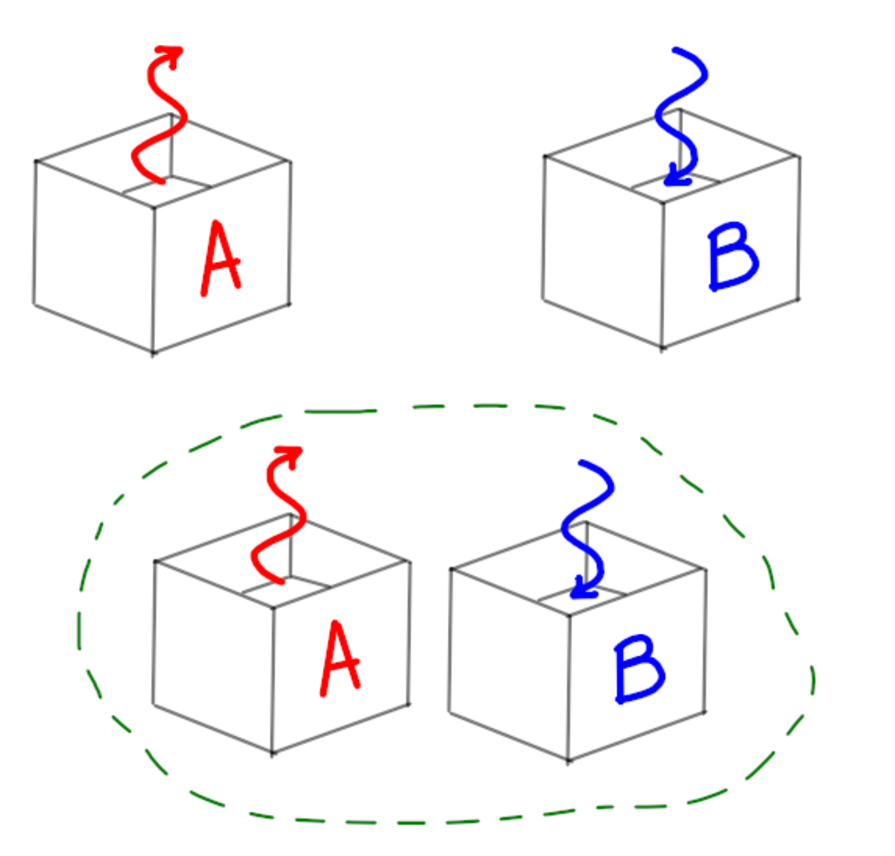
\includegraphics[width=0.3\linewidth]{cartoon1.pdf}
\captionof{figure}{If there are two subsystems, call them A and B, and both subsystems are in contact with the outside environment, where the set-up is that the subsystem A gains energy while subsystem B loses the same amount of energy. Then we can consider the A and B subsystems as time-reversed versions of each other. Taken together as a larger combined system, then the AB system has no net probability flux. Notice that when we exchange A for B there is no change to the composite system, This means that the combined AB system is \PT-symmetric.}
\label{fig:AB}
\end{Figure}
The parity operator \PP\ is defined as a linear, reflection operator. We can write a matrix representation of \PP\ to use in our above toy example:
\begin{equation} \label{eq:2}
P = \begin{bmatrix}
0 & 1 \\ 
1 & 0
\end{bmatrix}.
\end{equation}
Notice that $P^2 = 1$ and that the \PP-operator is equal to its inverse $P = P^{-1}$.
The time-reversal symmetry operator ($T$) is defined as antilinear in order to preserve the Heisenberg commutation relation $[\hat{x}, \hat{p}] = i\hbar$\cite{BenderPT} and thus be consistent with the time dependent Schrödinger equation\cite{Jones-Smith}.
The antilinearity of $T$ is defined as 
\begin{equation} \label{eq:3}
T \psi T^{-1}= L \psi^{*}.
\end{equation}
$T$ acts as complex conjugation of a state $\psi$ followed by a linear operator $L$ (which may or not be Hermitian) acting on the state. There are two kinds of time-reversal: Even and odd, that is $T^2 = 1$ and $T^2 = -1$ respectively. These two kinds of time-reversal symmetry apply to different particles. In the case of Bosons (integer spin) only even \TT-symmetry applies. while odd \TT-symmetry applies exclusively to Fermions (half-integer spin)\cite{Jones-Smith}.
The scope of this work will focus exclusively in the case of even \TT-symmetry. With this simplification we can work with a basis such that 
\begin{equation} \label{eq:4}
T \psi T^{-1} = \psi^{*}.
\end{equation}
By focusing on even \TT-symmetry we can consider $T$ as a reflection operator as we do with $P$. The \TT\ operator doesn't have a spatial basis matrix representation.
Parity and time-reversal operation are independent of each other, therefore the $P$ and $T$ operators commute\cite{BenderPT}.

In Figure~\ref{fig:AB} above, we considered a very simple case of a composite \PT-symmetric system, where the composition involved combining a subsystem A with its time-reversed version B.
Let us imagine that A can be described with the simple $1 \times 1 $ Hamiltonian $H_{A} = [a+ib]$ where $a, b \in \mathds{R}$, since we established that B is simply the time-reversed version of A then B's Hamiltonian is $H_{B} = T (H_{A}) T^{-1} = [a-ib]$.

We can write the Hamiltonian of the composite AB system as the $2 \times 2$ Hamiltonian matrix
\begin{equation} \label{eq:5}
H_{\mathrm{AB}} = \begin{bmatrix}
a+ib & 0 \\ 
0 & a-ib
\end{bmatrix}.
\end{equation}
$H_{AB}$ is not Hermitian, but we can prove that it is \PT-symmetric:
\begin{equation} \label{eq:6}
PT(H_{\mathrm{AB}})T^{-1}P^{-1} = \begin{bmatrix}
0 & 1 \\ 
1 & 0
\end{bmatrix}
T
\begin{bmatrix}
a+ib & 0 \\ 
0 & a-ib
\end{bmatrix}
T^{-1}
\begin{bmatrix}
0 & 1 \\ 
1 & 0
\end{bmatrix},
\end{equation}

\begin{equation} \label{eq:7}
\therefore PT(H_{\mathrm{AB}})T^{-1}P^{-1} = \begin{bmatrix}
0 & 1 \\ 
1 & 0
\end{bmatrix}
\begin{bmatrix}
a-ib & 0 \\ 
0 & a+ib
\end{bmatrix}
\begin{bmatrix}
0 & 1 \\ 
1 & 0
\end{bmatrix}
\end{equation}

\begin{equation} \label{eq:8}
\therefore PT(H_{\mathrm{AB}})T^{-1}P^{-1} = 
\begin{bmatrix}
a+ib & 0 \\ 
0 & a-ib
\end{bmatrix}
\end{equation}

\begin{equation} \label{eq:9}
\therefore PT(H_{\mathrm{AB}})T^{-1}P^{-1} = H_{\mathrm{AB}}.
\end{equation}
The system described by equation (\ref{eq:5}) is not in dynamic equilibrium, as time evolves the norm of the states of subsystem A decay and those of B grow. If we introduce a coupling parameter $g$ between our subsystems ($g$ can be complex), then the states of A and B will be coupled and so we can write the composite coupled-state Hamiltonian as 
\begin{equation} \label{eq:10}
H_{\mathrm{coupled}} = 
\begin{bmatrix}
a+ib & g \\ 
g & a-ib
\end{bmatrix}.
\end{equation}
Notice that \PT-symmetry is preserved in equation (\ref{eq:10}). The coupling strength $g$ determines the reality of the eigenvalue spectrum of $H_{\mathrm{coupled}}$.
To see this, we solve the eigenvalue problem
\begin{equation} \label{eq:11}
\mathrm{det}(H_{\mathrm{coupled}}-IE) = a^2 +b^2 + E^2 -g^2 -2aE,
\end{equation}
where $I$ is the identity matrix and $E$ are the real eigenvalues we want to find. Notice that the second order polynomial in equation (\ref{eq:11}) is real for any value of $g$. The roots of this polynomial are 
\begin{equation} \label{eq:12}
E_{\pm} = a \pm \sqrt{g^2 - b^2}.
\end{equation}
From this we can derive 3 scenarios. The first corresponds to the case when $g^2 < b^2$. In this case we have complex-valued eigenvalues, and so the weak coupling scenario yields a system that is not in dynamic equilibrium, because the coupled states continue to decay or grow. Alternatively, if $g^2 > b^2$ then this corresponds to strongly coupled states that do not decay nor grow, and so we have a real valued energy spectrum. These two coupling scenarios correspond to the cases of broken and unbroken \PT-symmetry respectively. Finally the last case is when $g = \pm b$. This is the degenerate case. In non-Hermitian systems, degeneracy is expressed by real eigenvalues merging into complex conjugate pairs as $|g| \rightarrow b$. In my discussion in section \ref{Experimental} I will explain on how the merging of eigenvalues has important experimental consequences.
%%%%%%%%%%%%%%%%%%%%%%%%%%%%%%%%%%%%%%%%%%%%%%%%%%%%%%%%%%%%%%%%%%%%%%%%%%%%%%%%%%%%%%%%%%%%%%%%%%%%%%%%%%%%%%%%%%%%%%%%%%%%%%%%%%%%%%%%%%%%%%%%%%%%%%%%%%%%%%%%%%%%%%%%%%%%%

\section{Nerd-Sniped}\label{Nerd}
\begin{Figure}
\centering
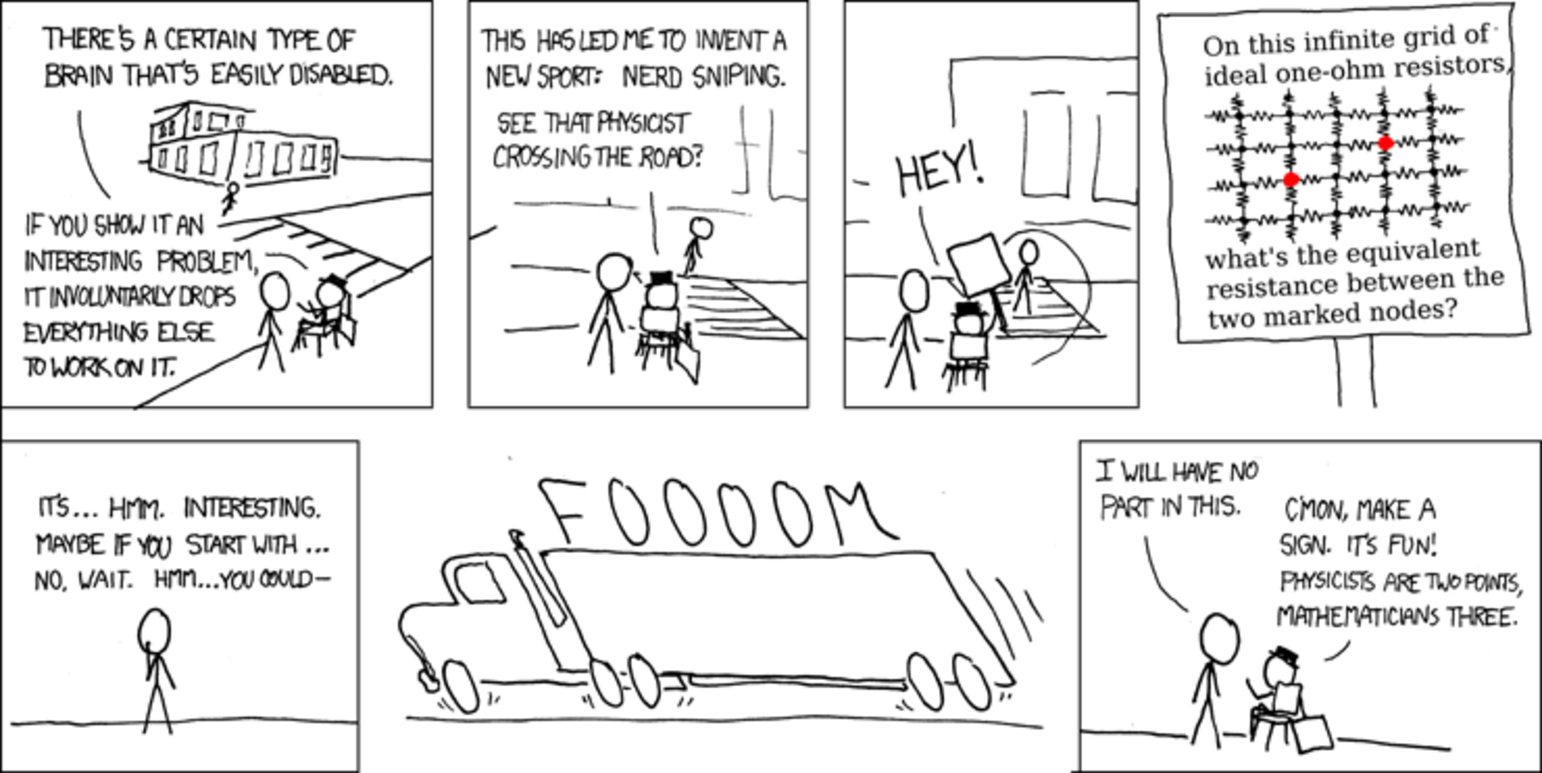
\includegraphics[width=\linewidth]{nerd_sniping.pdf}
\captionof{figure}{The relevant XKCD comic -Nerd Sniping (modified)- https://xkcd.com/356/. Illustrates what happened to me during my project. }
\end{Figure}
I must be honest, I had a couple of ideas for my project but I only achieved one of them. Early on in the semester while I was reading ``Making sense of non-Hermitian Hamiltonians'' by Carl Bender I encountered a really interesting figure.

\begin{Figure}
\centering
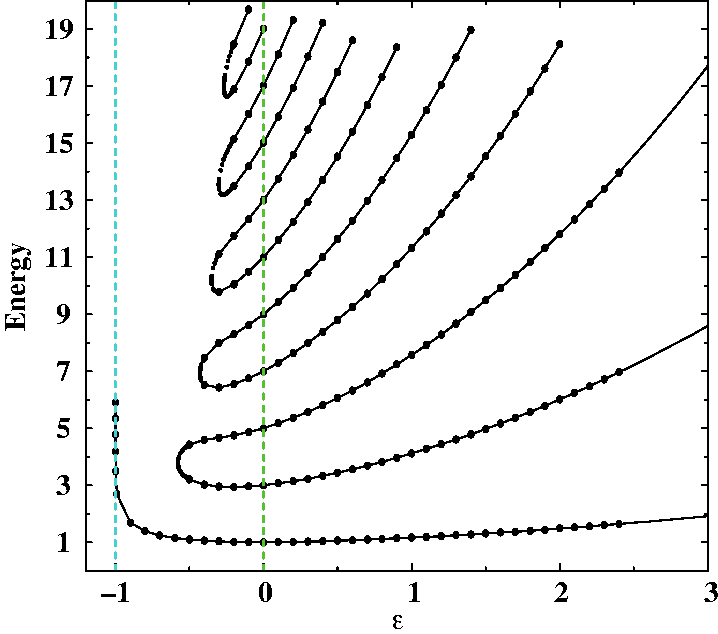
\includegraphics[width=0.65\linewidth]{figure_1_Bender.pdf}
\captionof{figure}{This is Figure 1. in reference \cite{Bender}.This figure exemplifies the behaviour of the eigenvalue spectra of the general parametric family of non-Hermitian Hamiltonians $\hat{H} = \hat{p}^2 + \hat{x}^2 (i \hat{x})^{\epsilon}$ as a function of the real parameter $\epsilon$. All the eigenvalues visible in this figure are real valued. The \PT-symmetry breaks at the $\epsilon = 0$, which corresponds to the Hamiltonian for the classic one dimensional harmonic oscillator. When $\epsilon \geq 0$ the spectra are real, positive and discrete. Energy levels increase with increasing $\epsilon$. In the region corresponding to $-1 \leq \epsilon \leq 0$ there is a finite number of real positive eigenvalues and an infinite number of complex-conjugate pairs of eigenvalues (not depicted). The number of real eigenvalues decreases as $\epsilon$ decreases from $0$ to $-1$, for $\epsilon$ that are more negative than the value $\epsilon = -0.57793$ the only remaining real eigenvalue corresponds to the ground-state energy. At the value $\epsilon = -1$ the spectrum is null (see image below for more details).}
\label{fig:Benders}
\end{Figure}

\begin{Figure}
\centering
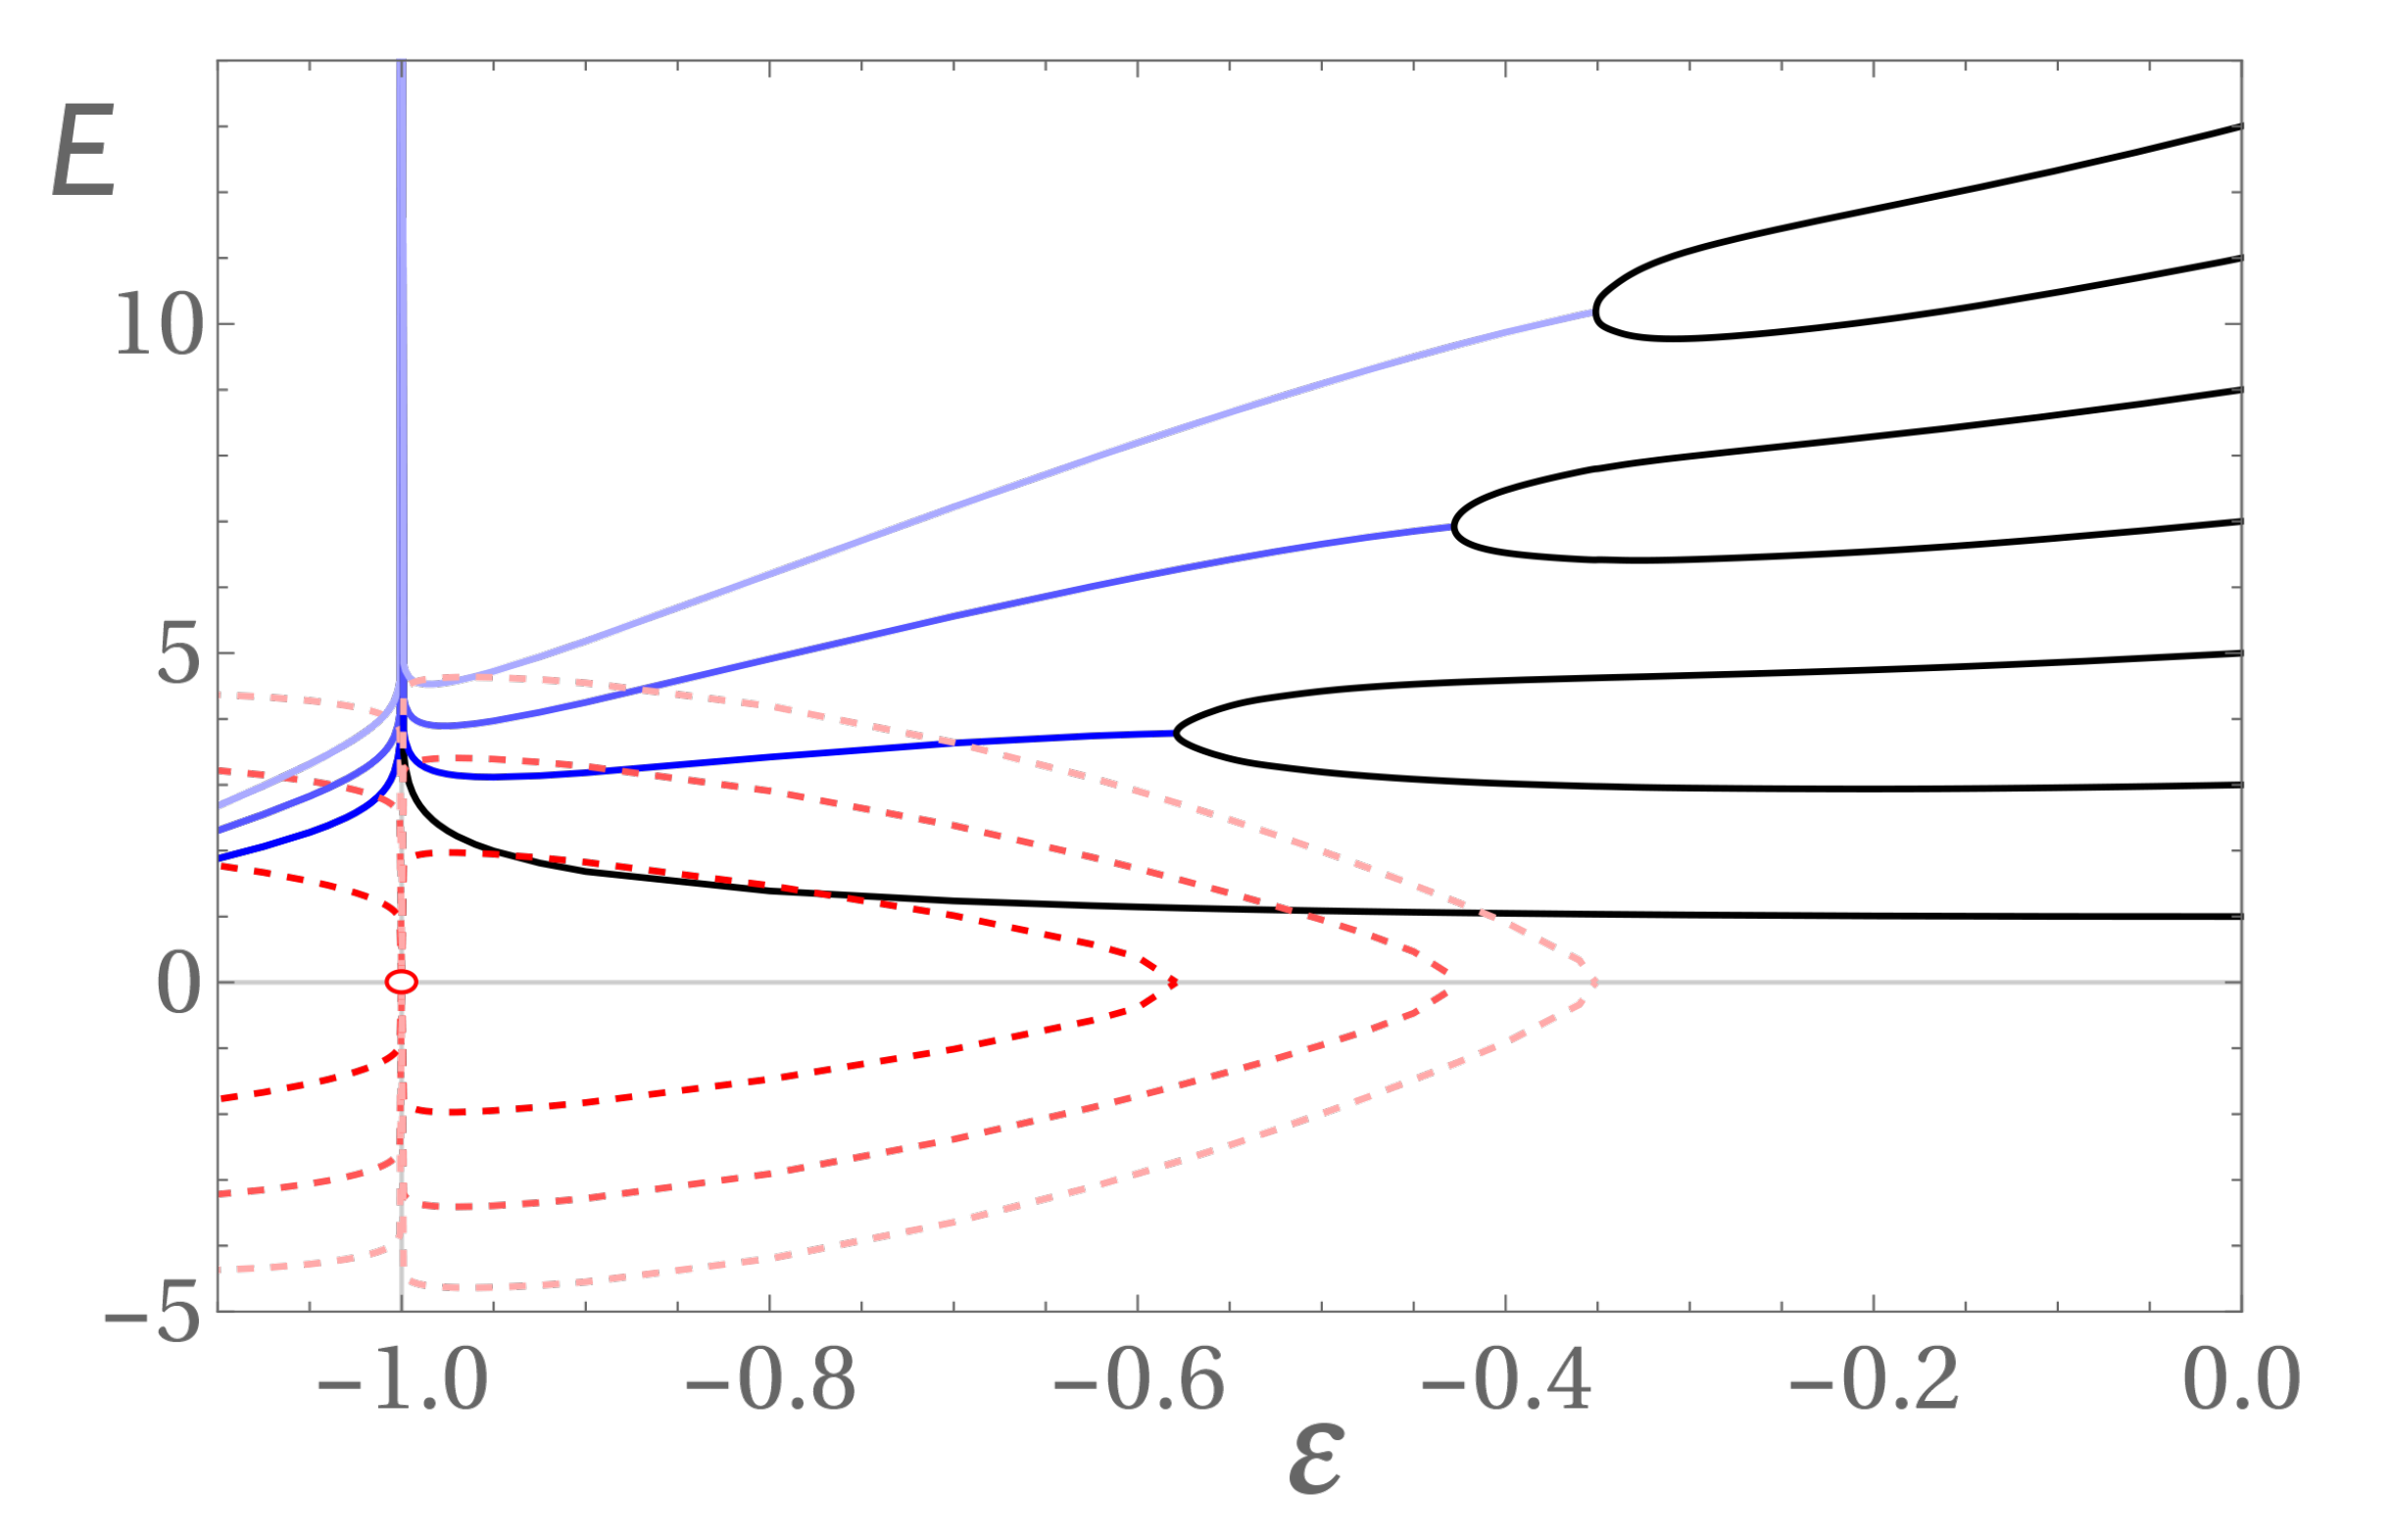
\includegraphics[width=0.75\linewidth]{figure_3_Bender_ET_AL.png}
\captionof{figure}{This is Figure 3. in reference \cite{Bender2017}. This figure exemplifies the behaviour of the eigenvalue spectra of the general parametric family of non-Hermitian Hamiltonians $\hat{H} = \hat{p}^2 + \hat{x}^2 (i \hat{x})^{\epsilon}$ as a function of the real parameter $\epsilon$ in the region corresponding to $-1 \leq \epsilon \leq 0$. In this region there are a finite number of real positive eigenvalues and an infinite number of complex-conjugate pairs of eigenvalues (only 3 conjugate pairs are depicted). The number of real eigenvalues decreases as $\epsilon$ decreases from $0$ to $-1$, for values of $\epsilon$ that are more negative than $\epsilon = -0.57793$ the only remaining real eigenvalue corresponds to the ground-state energy. At the value $\epsilon = -1$ the spectrum is null, as all the eigenvalues (real or real-parts) diverge to infinity, while the imaginary parts of the complex eigenvalues go to zero.}
\label{fig:Benders}
\end{Figure}

In the figures above, we can see how different the behaviour of the eigenvalues is in the region with unbroken \PT-symmetry from the region with broken \PT-symmetry.
\PT-symmetry is characterized by the commutation relation a Hamiltonian and the \PT-operator. The \PT-operator is non-linear, therefore the eigenstates of the Hamiltonian may or may not be eigenstates of the \PT-operator. 

The meaning of broken and unbroken \PT-symmetry can be written as the following conditional statement: \emph{If the Hamiltonian and the \PT-operator share all eigenstates, then the symmetry is \textbf{unbroken}, but if not all the eigenstates are simultaneously shared between the Hamiltonian and the \PT-operator then the symmetry is \textbf{broken}}\cite{BenderPT}\cite{Bender}. In other words, only if the \PT-symmetric Hamiltonian shares eigenstates with the \PT-operator, then the corresponding eigenvalues to those shared eigenstates are real-valued.

My investigations of non-Hermitian Hamiltonians were pivoted by trying to understand what was going on in the figure above. My approach was based on trying to replicate the figure itself as it portrays a very clear visualisation of \PT-symmetry breaking (occurring at $\epsilon = 0$) and its effect on the energy spectrum of the non-Hermitian \PT-symmetric Hamiltonians $\hat{H} = \hat{p}^2 + \hat{x}^2 (i \hat{x})^{\epsilon}$. Visible in this figure is the preservation of the reality and boundedness (from below) of the eigenvalues of Hamiltonians (with unbroken \PT symmetry) as the perturbation parameter $\epsilon$ varies. This result is certainly non-trivial, and it is crucial to the applicability of \PT-symmetry as a postulate of quantum theory.

For my investigation of this figure, I solved the time independent eigenvalue problems associated with a $\hat{H} = \hat{p}^2 + \hat{x}^2 (i \hat{x})^{\epsilon}$. In this work I use two different mathematical techniques, one of these is a complex extension of the well known WKB approximation, and the other is matrix Diagonalisation.

Replicating this figure took most of my time during the semester, and so I was unable to develop my other investigations further. Nevertheless, for the sake of completeness, I will describe in section \ref{Aborted} what my other project idea was.

%%%%%%%%%%%%%%%%%%%%%%%%%%%%%%%%%%%%%%%%%%%%%%%%%%%%%%%%%%%%%%%%%%%%%%%%%%%%%%%%%%%%%%%%%%%%%%%%%%%%%%%%%%%%%%%%%%%%%%%%%%%%%%%%%%%%%%%%%%%%%%%%%%%%%%%%%%%%%%%%%%%%%%%%%%%%%

\chapter{Numerical determination of eigenstates and eigenvalues of non-Hermitian Hamiltonians}\label{Benders}
The defining principle behind Figure~\ref{fig:Benders} on page~\pageref{fig:Benders} is that we can think of the family of non-Hermitian \PT-symmetric Hamiltonians defined below as complex deformations of the Hermitian and \PT-symmetric 1D classical harmonic oscillator
\begin{equation}\label{eq:17}
\hat{H} = \hat{p}^2 + \hat{x}^2 (i \hat{x})^{\epsilon},
\end{equation}
where $\epsilon$ is a real parameter. The introduction of the real parameter $\epsilon$ acts in such a way that as $\epsilon$ increases from $0$, the Hamiltonian is no longer Hermitian but its \PT-symmetry is preserved. This occurs because the quantity $(i\hat{x})$ is \PT-invariant\cite{BenderPT}\cite{Bender}.
To formulate the eigenvalue problems for both methods used to find all the eigenvalues of equation (\ref{eq:17}), I split the problem into the expected parametric regions (as per Bender's descriptions) corresponding to \emph{unbroken} \PT-symmetry ($\epsilon \geq 0$) and \emph{broken} \PT-symmetry ($\epsilon < 0$).
When $\epsilon \geq 0$ the eigenvalues are real, positive, discrete and energy levels increase with increasing $\epsilon$.
To solve the Schrödinger eigenvalue problem I wrote the Schrödinger equation in coordinate space. The relevant operators in this space are
\begin{align} \label{eq:18}
\hat{x}& \rightarrow x, &\hat{p}\rightarrow -i \frac{d}{dx},
\end{align}
where we want to treat the variable x as complex. Notice that this does not modify the commutation relation $[\hat{x}, \hat{p}] = i\hbar$. Also, without loss of generality we can use natural length scales $(\hbar = 1, m = \frac{1}{2})$ so the eigenvalue problem takes the form
\begin{equation}\label{eq:19}
-\psi'' + x^2 (i x)^{\epsilon} \psi = E \psi.
\end{equation}
Equation (\ref{eq:19}) cannot be solved exactly using analytic methods for $\epsilon \neq 0$, therefore my approach is numerical. From reference \cite{Bender} I learned that the WKB phase integral approximation can be used to find very a accurate approximation to the real eigenvalues visible in the \emph{unbroken} \PT-symmetry region ($\epsilon \geq 0$) in Figure~\ref{fig:Benders} on page~\pageref{fig:Benders}. 
%%%%%%%%%%%%%%%%%%%%%%%%%%%%%%%%%%%%%%%%%%%%%%%%%%%%%%%%%%%%%%%%%%%%%%%%%%%%%%%%%%%%%%%%%%%%%%%%%%%%%%%%%%%%%%%%%%%%%%%%%%%%%%%%%%%%%%%%%%%%%%%%%%%%%%%%%%%%%%%%%%%%%%%%%%%%%

\section{Methods}
\subsection{WKB approximation}\label{WKB}
To solve equation (\ref{eq:19}) I had to find out which were the boundary conditions for the problem. I learned from several sources that the boundary conditions depend on the deformation parameter $\epsilon$ \cite{BenderPT}\cite{Bender}\cite{Bender2017}. Since the eigenvalue problem can be conceptualised as a harmonic oscillator that has been deformed into the complex x-plane, we must re-frame the spatial variable $x$ as $x = r e^{i\theta}$. Finding the solutions requires that I integrate equation (\ref{eq:19}) along a contour in the complex x-plane and that the solution be equal to zero at both ends of this contour\cite{BenderPT}, i.e. the eigenfunctions vanish exponentially for large $|x|$. According to Bender, the integration contour should be located within two angular sectors in the complex x-plane. These sectors are called \emph{Stokes wedges}\cite{BenderPT}\cite{Bender}, in general these wedges are centred about the origin in the complex x-plane and we can define their orientation in terms of the $Arg(x) = \theta$ as follows
\begin{align} \label{eq:20}
&-\frac{1}{4} \pi < \theta < \frac{1}{4}\pi& &\mathrm{and}& &\frac{3}{4} \pi < \theta < \frac{5}{4}\pi.& 
\end{align}
For my eigenvalue problem, it is required to understand the asymptotic behaviour of the solutions for large $|x|$ values.\\
In my method, I assumed that for an ODE of the form of equation (\ref{eq:19}), the behaviour of $E - V(x) \rightarrow \infty$ as $|x| \rightarrow \infty$ in the complex x-plane. The next assumption I made was that the solution should be
\begin{equation} \label{eq:21}
\psi \sim \mathrm{exp}[\pm \int^{x}dx \sqrt{E - V(x)}],
\end{equation}
this approximation solution is known as the \emph{geometrical-optics approximation}\cite{BenderPT}.

The location of \emph{Stokes wedges} in the complex plane, and hence the defined boundary conditions for my problem are determined by imposing that \mbox{$\psi(x) \rightarrow 0$ as $|x| \rightarrow \infty$} similarly to the case where $\epsilon = 0$, i.e. the classical harmonic oscillator case, where the solutions are known to be square integrable for real x-values.

Since I am assuming that my solutions will be wave functions moving in space, I am interested in learning how much phase is gained by traversing the integration contour in the complex x-plane. The end points of the integration contour are the turning points (the roots of the equation $E = x^2(ix)^{\epsilon}$) that \emph{analytically continue off} of the real axis as $\epsilon$ increases from $0$\cite{BenderPT}\cite{Bender}. Independently of the number of possible roots of $E = x^2(ix)^{\epsilon}$, for the purpose of my technique I only need the following turning points to be the limits of integration
\begin{align} \label{eq:22}
x_{-}& = 
E^{\frac{1}{\epsilon + 2}}
e^{i\pi(\frac{3}{2} - \frac{1}{\epsilon + 2})}
&\mathrm{and}&
&x_{+} = E^{\frac{1}{\epsilon + 2}} e^{-i\pi(\frac{1}{2} - \frac{1}{\epsilon + 2})}.
\end{align}
The explicit formula I used in my numerical calculation of the eigenvalues is the the leading order WKB phase integral quantization condition 
\begin{equation} \label{eq:23}
\left (n +\frac{1}{2}\right )\pi = \int^{x_{+}}_{x_{-}}dx \sqrt{E - x^2(ix)^{\epsilon}}.
\end{equation}
In ``Making sense of non-Hermitian Hamiltonians'', Bender describes equation (\ref{eq:23}) as the quantization condition on the accumulated phase integral that defines the energy.

Since the standard Python numerical libraries do not support complex integration, I proceeded with my numerics by implementing a change of variables that shifted my integration limits and domain from the complex plane to the real line. I did this because both turning points $x_{\pm}$ have equal imaginary parts, I subtracted the imaginary part multiplied by $i$ from both of the integration limits and also added it to the complex $x$ value present in the integrand as an offset
\begin{equation} \label{eq:24}
\begin{split}
&x_{-}\rightarrow x_{-}' = x_{-} - i \mathrm{Im}(x_{-}),\\
&x_{+}\rightarrow x_{+}' = x_{+} - i \mathrm{Im}(x_{-}),\\
&x\rightarrow x = x' - i \mathrm{Im}(x_{-}),\\
&dx\rightarrow dx'.
\end{split}
\end{equation}

After my change of variables, I was able to calculate the WKB integral by writing my own integration function and using the \texttt{scipy,integrate.quad()} module for integration in Python. I wrote a modified function that calculated the integral for the real part and the integral for imaginary part of the integrand separately and set the function to return the total integral as a linear combination of the real plus $i$ times the imaginary part. I named my function: \texttt{complex\_quad()}.

I was able to verify the quantisation condition in equation (\ref{eq:23}) by taking the difference of the expression dependent of n in the left hand side of equation (\ref{eq:23}) and the complex integral corresponding to the right hand side of equation (\ref{eq:23}).
I used this difference equation to optimize the resulting energy eigenvalue from my \texttt{complex\_quad()} function. For the optimization I used my own modified version of the root finding algorithm module \texttt{scipy.optimize.fsolve()}. My modifications simply allowed me to use the algorithm for both the real and imaginary part of my results, and to combine them similarly to what I did when calculating the real and imaginary parts of the complex integral as two separate integrals.
%%%%%%%%%%%%%%%%%%%%%%%%%%%%%%%%%%%%%%%%%%%%%%%%%%%%%%%%%%%%%%%%%%%%%%%%%%%%%%%%%%%%%%%%%%%%%%%%%%%%%%%%%%%%%%%%%%%%%%%%%%%%%%%%%%%%%%%%%%%%%%%%%%%%%%%%%%%%%%%%%%%%%%%%%%%%%

\subsection{Matrix equations}\label{Matrix equations}
The process I followed to solve equation (\ref{eq:19}) for the region corresponding to values of $\epsilon < 0$ was a lot more free form than for the unbroken \PT-symmetry region. In ``Making sense of non-Hermitian Hamiltonians'' Bender didn't go into details about the behaviour of the spectrum this region nor gave any advice on how to solve the eigenvalue problem for the parametric Hamiltonians with $\epsilon < 0$ values. I chatted to my supervisors a lot when I was working on this and we settled on me attempting to re-write equation (\ref{eq:19}) as a matrix equation using the family of harmonic oscillators eigenstates written in the spatial coordinate the basis. These basis functions are also known as Hermite functions and are generally written as
\begin{align} \label{eq:25}
&\psi_n(x)= \frac{1}{\sqrt{2^n n!}} 
\left ( \frac{m \omega}{\pi \hbar}\right )^{1/4} e^{\frac{-m \omega x^2}{2 \hbar}}
H_n \left (\sqrt{\frac{m \omega}{\hbar}}x\right ), &n = 0, 1, 2, \dots
\end{align}
where the functions $H_n(z)$ are the physicists' Hermite polynomials
\begin{equation} \label{eq:26}
H_n(z) = (-1)^n e^{z^2} \frac{d^n}{dz^n}\left( e^{-z^2}\right).
\end{equation}
In equation (\ref{eq:19}) I have used natural length scales, i.e. $\hbar = 1, m = \frac{1}{2}$. To simplify my states further, I set the frequency in my harmonic oscillator basis states to $\omega = 2$ to obtain
\begin{equation} \label{eq:27}
\psi_n(x)= \frac{1}{\sqrt{2^n n!}} 
\left ( \frac{1}{\pi}\right )^{1/4} e^{\frac{-x^2}{2}}
H_n (x).
\end{equation}
To numerically diagonalise the Hamiltonian I first needed to numerically calculate $N$ (I chose $N = 100$) harmonic oscillator basis functions as they are written in equation (\ref{eq:27}), and then I used them to form the matrix elements 
\begin{equation}\label{eq:28}
\left \langle m \left |\hat{H} \right|n \right \rangle = \int_{-b}^{b} \psi_m(x)^* \left ( - \frac{d^2}{dx^2} + x^2(ix)^{\epsilon}\right ) \psi_n(x) dx,
\end{equation}
where $m$ and $n$ are the indices for harmonic oscillator states. Both $m, n$ range from 0 to 100, and $\pm b$ are the integration limits which I will define in the next section. Using these elements I constructed one hundred Hamiltonian matrices. Each Hamiltonian matrix corresponds to a different $\epsilon$ value in a range of one hundred values between $0$ and $-1$. 
After the matrices were constructed I simply used the \emph{scipy.linalg.eig()} module in Python to solve each eigenvalue problem for my set of $100\times100$ Hamiltonian matrices. With this module I found the eigenvalues and the right eigenvectors for each matrix.
%%%%%%%%%%%%%%%%%%%%%%%%%%%%%%%%%%%%%%%%%%%%%%%%%%%%%%%%%%%%%%%%%%%%%%%%%%%%%%%%%%%%%%%%%%%%%%%%%%%%%%%%%%%%%%%%%%%%%%%%%%%%%%%%%%%%%%%%%%%%%%%%%%%%%%%%%%%%%%%%%%%%%%%%%%%%%

\subsubsection{Matrix elements}\label{Matrix elements}
An important part of my integral calculations was the need to choose the integration region for each matrix element. I needed the largest possible region without compromising the computational time spent for each element integration. I concluded that the integration bounds must depend on the state with the highest energy value used for each of the one hundred elements calculated. In addition, I needed to make sure the wave functions went to zero for large $x$ values in order to take advantage of the behaviour of basis states for large $|x|$. I set the limits of integration to be much larger than the turning points of the harmonic oscillator, with this I was able to guarantee that the states have exponentially decayed to zero at the bounds of my integration. I settled the boundaries by trial and error and determined that the values $b = \pm \sqrt{4 \mathrm{min}(m,n) + 2} + 2$ were more than adequate.

To iteratively calculate the matrix elements as they are written in equation (\ref{eq:28}) I once again, used my \texttt{complex\_quad()} function since the integrand of each matrix element integral was complex-valued. My modified function calculates the integral for the real part and the integral for imaginary part of the integrand and returns the total integral as a linear combination of the real plus $i$ times the imaginary part.

Finally, my code repeated this procedure and calculated one hundred $100\times100$ matrices: one matrix for each $\epsilon$ in my discretised region for $\epsilon$ values between 0 and -1.

Constructing the integrand for each matrix element as per equation (\ref{eq:28}) was computationally expensive, because it required the calculation of the harmonic oscillator basis functions $\psi_m$ and $\psi_n$, and the application of the Hamiltonian. To numerically calculate the second order derivative in the Hamiltonian I used a finite centred differences approximation
\begin{equation}\label{eq:29}
\frac{d^2 \psi_n(x)}{dx^2} = \frac{\psi_n(x + h) - 2 \psi_n(x) + \psi_n(x - h)}{h^2}.
\end{equation}

I have $100\times100$ matrices. Each matrix calculation has complexity $O(N^2)$. Furthermore, calculating each basis function basis function for the matrix elements involves a recursion relation applied N times, so that's another factor of N. Therefore the total complexity of my algorithm is $O(N^3)$. I will explain now why this approach crashed my calculation on my first attempts.
%%%%%%%%%%%%%%%%%%%%%%%%%%%%%%%%%%%%%%%%%%%%%%%%%%%%%%%%%%%%%%%%%%%%%%%%%%%%%%%%%%%%%%%%%%%%%%%%%%%%%%%%%%%%%%%%%%%%%%%%%%%%%%%%%%%%%%%%%%%%%%%%%%%%%%%%%%%%%%%%%%%%%%%%%%%%%

\subsubsection{Hermite functions}\label{Hermite functions}
The main computational issue was due to the size of the Harmonic oscillator basis functions written in equation (\ref{eq:27}). The problem is specifically due to two of the factors that comprise the states. First, $\frac{1}{\sqrt{2^n n!}}$ \textbf{underflows} as n grows large, and the Hermite polynomial $H_n(x)$ \textbf{overflows} as n grows large. The behaviour of these factors makes numerically generating high n harmonic oscillator states an impossible feat (frustratingly, high n can be as low as n = 130).
I solved this problem using a modified version of a numerical method available in \url{www.numbercrunch.de/blog/2014/08/calculating-the-hermite-functions} by H. Bauke. The aim of the method is to calculate the functions in equation (\ref{eq:27}) using the recurrence relation 
\begin{equation} \label{eq:30}
H_n(x) = 2xH_{n-1}(x) - 2(n-1)H_{n-2}(x),
\end{equation}
where $H_0(x) = 1 $ and $H_1(x) = 2x$. The recursion relation partly eliminates the blow up of equation (\ref{eq:27}) by taking care of the issue due to large values of n. The method defines the recurrence relation corresponding to equation (\ref{eq:27}) as 
\begin{equation} \label{eq:31}
\psi_n(x) = \sqrt{\frac{2}{n}}x\psi_{n-1}(x) - \sqrt{\frac{n-1}{n}}(n-1)\psi_{n-2}(x).
\end{equation}
To fully solve all problems of underflow and overflow in equation (\ref{eq:27}), it is necessary to consider what happens when we are dealing with Hermite functions at large x values.

For $x>38$ the factor $\mathrm{e}^{-x^2/2}$ in equation (\ref{eq:27}) is smaller than any number that can be represented as a double precision floating point number. The general idea to fix numerical underflow due to large $|x|$ values is to keep the magnitude of the modified Hermite polynomials on the order of one during their calculation via the recurrence relation in (\ref{eq:31}), this is done by introducing a normalizing factor. During the calculation one has to keep track of the sum of the logarithms of these normalizing factors. Then the factor $\mathrm{e}^{-x^2/2}$ has to be modified by this sum when the value of the Hermite function is calculated. This algorithm allows to calculate the values of high-order Hermite functions even for quite large $|x|$ values.\cite{Bauke}.

Once I Implemented the changes to my code suggested by Bauke's work, my matrix elements could actually be computed without over/underflow, but the speed of each integral I calculated was incredibly slow. My numerics required some Cython to allow the code to compile the function using C in order to bypass the limitations that come from using exclusively Python. My partner Chris helped me with this step and he translated my recursion relation code into Cython for me. The algorithm is still the same complexity as before $(O(N^3))$ but the calculations were computed approximately $380\times$ faster than when I used Python code. Still, I had up to one hundred matrices to compute so I left the code running overnight.
%%%%%%%%%%%%%%%%%%%%%%%%%%%%%%%%%%%%%%%%%%%%%%%%%%%%%%%%%%%%%%%%%%%%%%%%%%%%%%%%%%%%%%%%%%%%%%%%%%%%%%%%%%%%%%%%%%%%%%%%%%%%%%%%%%%%%%%%%%%%%%%%%%%%%%%%%%%%%%%%%%%%%%%%%%%%%

\subsubsection{Visualising eigenstates in the broken \PT-symmetry region}\label{Eigenstates explained}
Jesper suggested that I make an animation to illustrate how the wave functions of the Hamiltonian in equation (\ref{eq:17}). change as $\epsilon$ changes in the energy-$\epsilon$ diagram. The the main motivations for creating this animation were: First, to verify if the eigenvectors were orthogonal, because the complex eigenstates of a non-Hermitian system are, in general, not orthogonal (for more on this, see Discussion section \ref{Orthogonal}); Second, because we wanted to observe the coalescent behaviour of the eigenvalues present in the broken symmetry region of the spectrum. We were particularly curious to see how an eigenfunction continuously becomes another, and we were also intrigued by the point at which this transformation would be visible.

For simplicity, I decided to exclusively use the first and second excited states for the Hamiltonian in equation (\ref{eq:17}). I chose these two wave function states because they certainly coalesce in Figure~\ref{fig:Benders} on page~\pageref{fig:Benders} and also in my own rendition of this figure (available in section \ref{Final}).

To find these specific eigenstates I had to extract the second and third eigenstates from the eigenstate list using the indices of the second and third elements of the sorted eigenvalues list (these lists were obtained by applying the \texttt{scipy.linalg.eig()} module to each of my Hamiltonian matrices). To sort the eigenvalues list, I used Boolean arrays to conditionally select the eigenvalues that satisfied some filtering condition. I filtered all the eigenvalues by requiring that the real-parts were $0< \mathrm{Re}(E) < 20$. I also indexed the eigenstates list using this filter, this works because the originally unsorted eigenvalues and eigenstates lists are organised in the same unsorted way.

After this, I sorted the filtered eigenstates by using \texttt{numpy.argsort()} on the unsorted filtered eigenvalues list to return the indices that would sort the array based on the newly sorted and filtered eigenvalue array. The \texttt{numpy.argsort()} function performs an indirect sort along the given axis using the algorithm specified by a keyword. My sorting keyword used the rounded real-part of the eigenvalues up to 3 significant figures plus the scaled (by $\frac{1}{10^6}$) rounded imaginary-part of the eigenvalues up to 3 significant figures. This condition made the sorting principally influenced by the real-part of the eigenvalue and only influenced by the imaginary part if the real parts were exactly equal. The \texttt{numpy.argsort()} function returns an array of indices of the same shape as a that index data along the given axis in sorted order\cite{argsort}.

After the filtering and sorting of eigenstates, I normalised the wave function states by 
\begin{equation}
\psi_{j}(x_{i}) = \frac{\psi_{j}(x_{i})}{\sqrt{\sum_{i} |\psi(x_{i})|^2 \Delta x}},
\end{equation}
where $\psi(x_{i})$ are the individual points forming the wave function.

Since the eigenstates might be returned with an arbitrary phase, to avoid ugly discontinuities in my plot frames I eliminated these arbitrary phases by multiplying the state by the exact opposite phase factor.
\begin{equation}
\psi_{j}(x_{i}) = \psi_{j}(x_{i}) e^{-i\mathrm{Arg}(\psi_{j}(x_{i})}.
\end{equation}

Finally, I obtained one hundred plots that were to be used as frames for my animation of the second and third eigenstates of the Hamiltonian in equation (\ref{eq:17}). I also made another animation of the probability amplitudes of the wave function eigenstates. I showed the probability amplitudes animation during my oral presentation.
\vspace*{5cm}
%%%%%%%%%%%%%%%%%%%%%%%%%%%%%%%%%%%%%%%%%%%%%%%%%%%%%%%%%%%%%%%%%%%%%%%%%%%%%%%%%%%%%%%%%%%%%%%%%%%%%%%%%%%%%%%%%%%%%%%%%%%%%%%%%%%%%%%%%%%%%%%%%%%%%%%%%%%%%%%%%%%%%%%%%%%%%

\section{Results}
\subsection{The region of unbroken \PT-symmetry}\label{PT unbroken}
Using equation (\ref{eq:23}), I calculated how much phase is gained by traversing a contour in the complex plane from one of the turning points in equation (\ref{eq:23}) to the other. Here I compare my numerical results for the energies pertaining to the unbroken \PT-symmetry region $(\epsilon \geq 0)$ in Figure~\ref{fig:Benders} on page~\pageref{fig:Benders} with the energies reported in Bender's paper ``Making sense of non-Hermitian Hamiltonians''. I plotted my obtained energy values together with Bender's values which are reported to have been obtained by the WKB integral and by Runge-Kutta.
\begin{Figure}
\centering
\hspace*{-1.7cm}
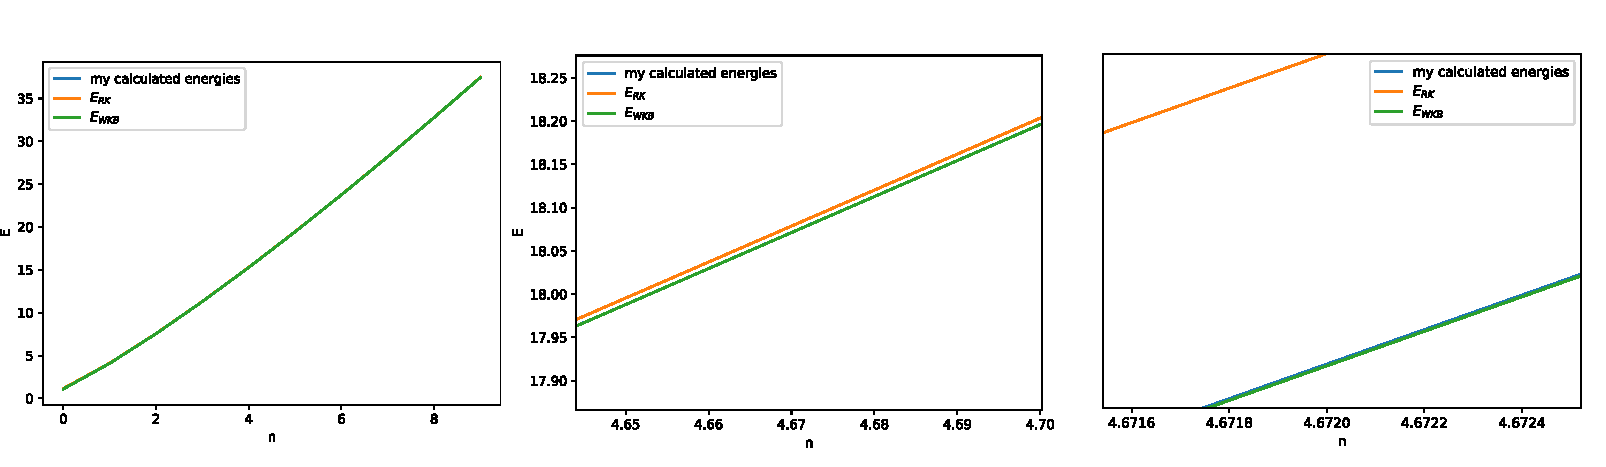
\includegraphics[width=1.2\linewidth]{comparing_to_bender(4).pdf}
\captionof{figure}{Plots of energy eigenvalues corresponding to the non-Hermitian \PT-symmetric Hamiltonian $\hat{H} = \hat{p}^2 + \hat{x}^2 (i \hat{x})$ (i.e. the case: $\epsilon = 1$ for equation (\ref{eq:17}), increasing in zoom level from top to bottom. For all plots, the vertical axis is energy and the horizontal axis corresponds to $n$. Here I demonstrate that my WKB energy results (blue plot) are in agreement with the energy values reported in Bender's work. Bender's results were obtained by the Runge-Kutta method (orange plot) and by the WKB approximation (green plot). All the energies presented in this plot were obtained using $n \in [0,9]$.}
\end{Figure}
\begin{Figure}
\centering
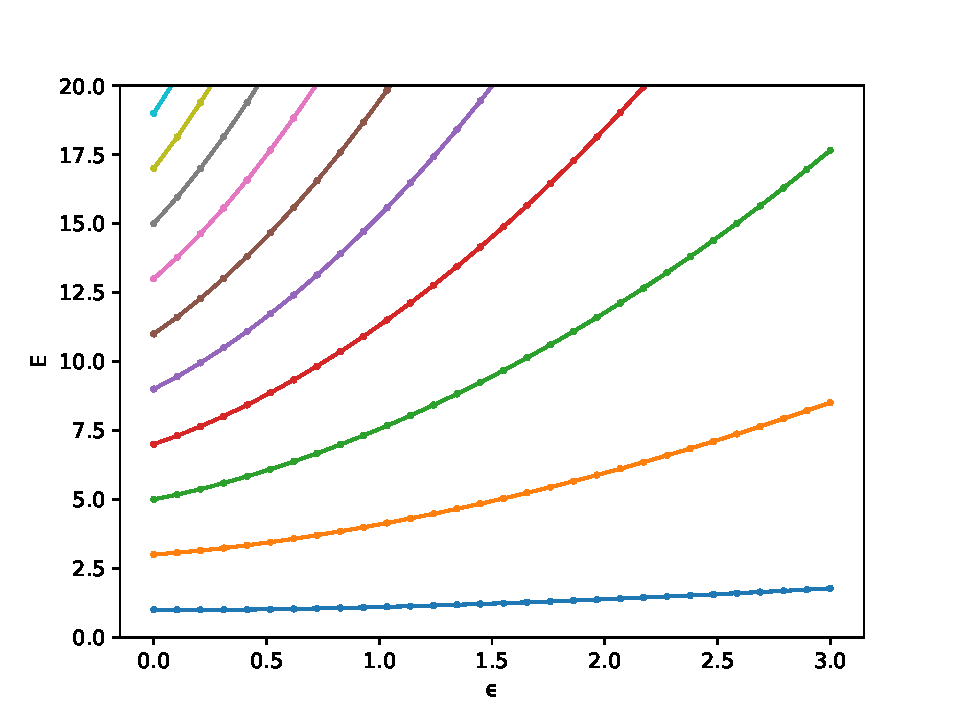
\includegraphics[width=0.8\linewidth]{unbroken_symmetry.pdf}
\captionof{figure}{My implementation of the WKB method on the family of non-Hermitian, \PT-symmetric Hamiltonians in equation (\ref{eq:17}), for positive $\epsilon$ values. The horizontal axis is the range of values $0 \leq \epsilon \leq 3$ and the vertical axis is the eigen-energy range $0 \leq E \leq 20$. My energy values are in agreement with those visible in Figure~\ref{fig:Benders} on page~\pageref{fig:Benders}. All the energies presented in this plot are real valued, and they are bounded below by the eigenvalues corresponding to the ground-state for each $\epsilon$ dependent Hamiltonian in equation (\ref{eq:17}) (visible as the lowest energies in the blue graph).The changing colours of every plot represent increasing values of n corresponding to the left hand side expression in the WKB quantisation condition (equation (\ref{eq:23}))}
\end{Figure}
%%%%%%%%%%%%%%%%%%%%%%%%%%%%%%%%%%%%%%%%%%%%%%%%%%%%%%%%%%%%%%%%%%%%%%%%%%%%%%%%%%%%%%%%%%%%%%%%%%%%%%%%%%%%%%%%%%%%%%%%%%%%%%%%%%%%%%%%%%%%%%%%%%%%%%%%%%%%%%%%%%%%%%%%%%%%%
\vspace*{12cm}
\subsection{The region of broken \PT-symmetry}\label{PT broken}
I solved the eigenvalue problem presented in equation (\ref{eq:19}) for one hundred different parametric Hamiltonians as per equation (\ref{eq:17}). I obtained my numerical results for the eigenvalue spectra of each Hamiltonian for one of the $\epsilon$ values in the discretised range of a hundred values ranging from 0 to -1. My obtained energy values matched the plotted energies reported in Bender’s paper “Making sense of non-Hermitian Hamiltonians”, and Bender et al. ``Behaviour of eigenvalues in a region of broken PT symmetry''.
\begin{Figure}
 \centering
 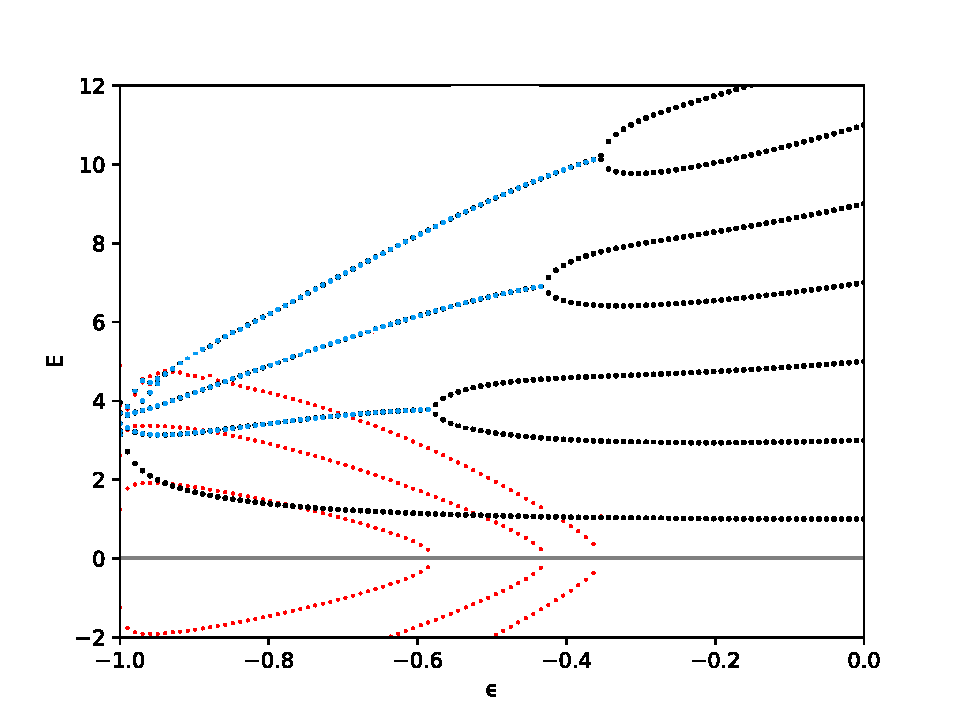
\includegraphics[width=\linewidth]{broken_region.pdf}
 \captionof{figure}{This plot is an extension of Figure~\ref{fig:Benders} on page~\pageref{fig:Benders}. This figure depicts the eigenvalues of the parametric family of Hamiltonians in equation (\ref{eq:17}) for the region corresponding to $\epsilon \leq 0$ . Here I display a discretised  parameter space for $\epsilon$ as 100 values in the horizontal axis, and the eigen-energy range $-2 \leq E \leq 12$ as the vertical axis. This figure depicts fully real eigenvalues as black dots. Visible here are three epsilon values at which the real eigenvalues become degenerate (coalesce) and then form complex-conjugate pairs. The real parts of these pairs of eigenvalues are represented as blue dots. These initially decrease as $\epsilon$ decreases but blow up suddenly as $\epsilon$ approaches -1 (The blow up of the real-parts was not captured by my numerics). The imaginary parts of the eigenvalue pairs are represented as red dots. These remain finite and appear to decay to zero at $\epsilon = -1$.}
\end{Figure}

%%%%%%%%%%%%%%%%%%%%%%%%%%%%%%%%%%%%%%%%%%%%%%%%%%%%%%%%%%%%%%%%%%%%%%%%%%%%%%%%%%%%%%%%%%%%%%%%%%%%%%%%%%%%%%%%%%%%%%%%%%%%%%%%%%%%%%%%%%%%%%%%%%%%%%%%%%%%%%%%%%%%%%%%%%%%%
\subsection{The behaviour of eigenstates}\label{Eigenstates}

\begin{Figure}
 \centering
 \hspace*{-0.9cm}
 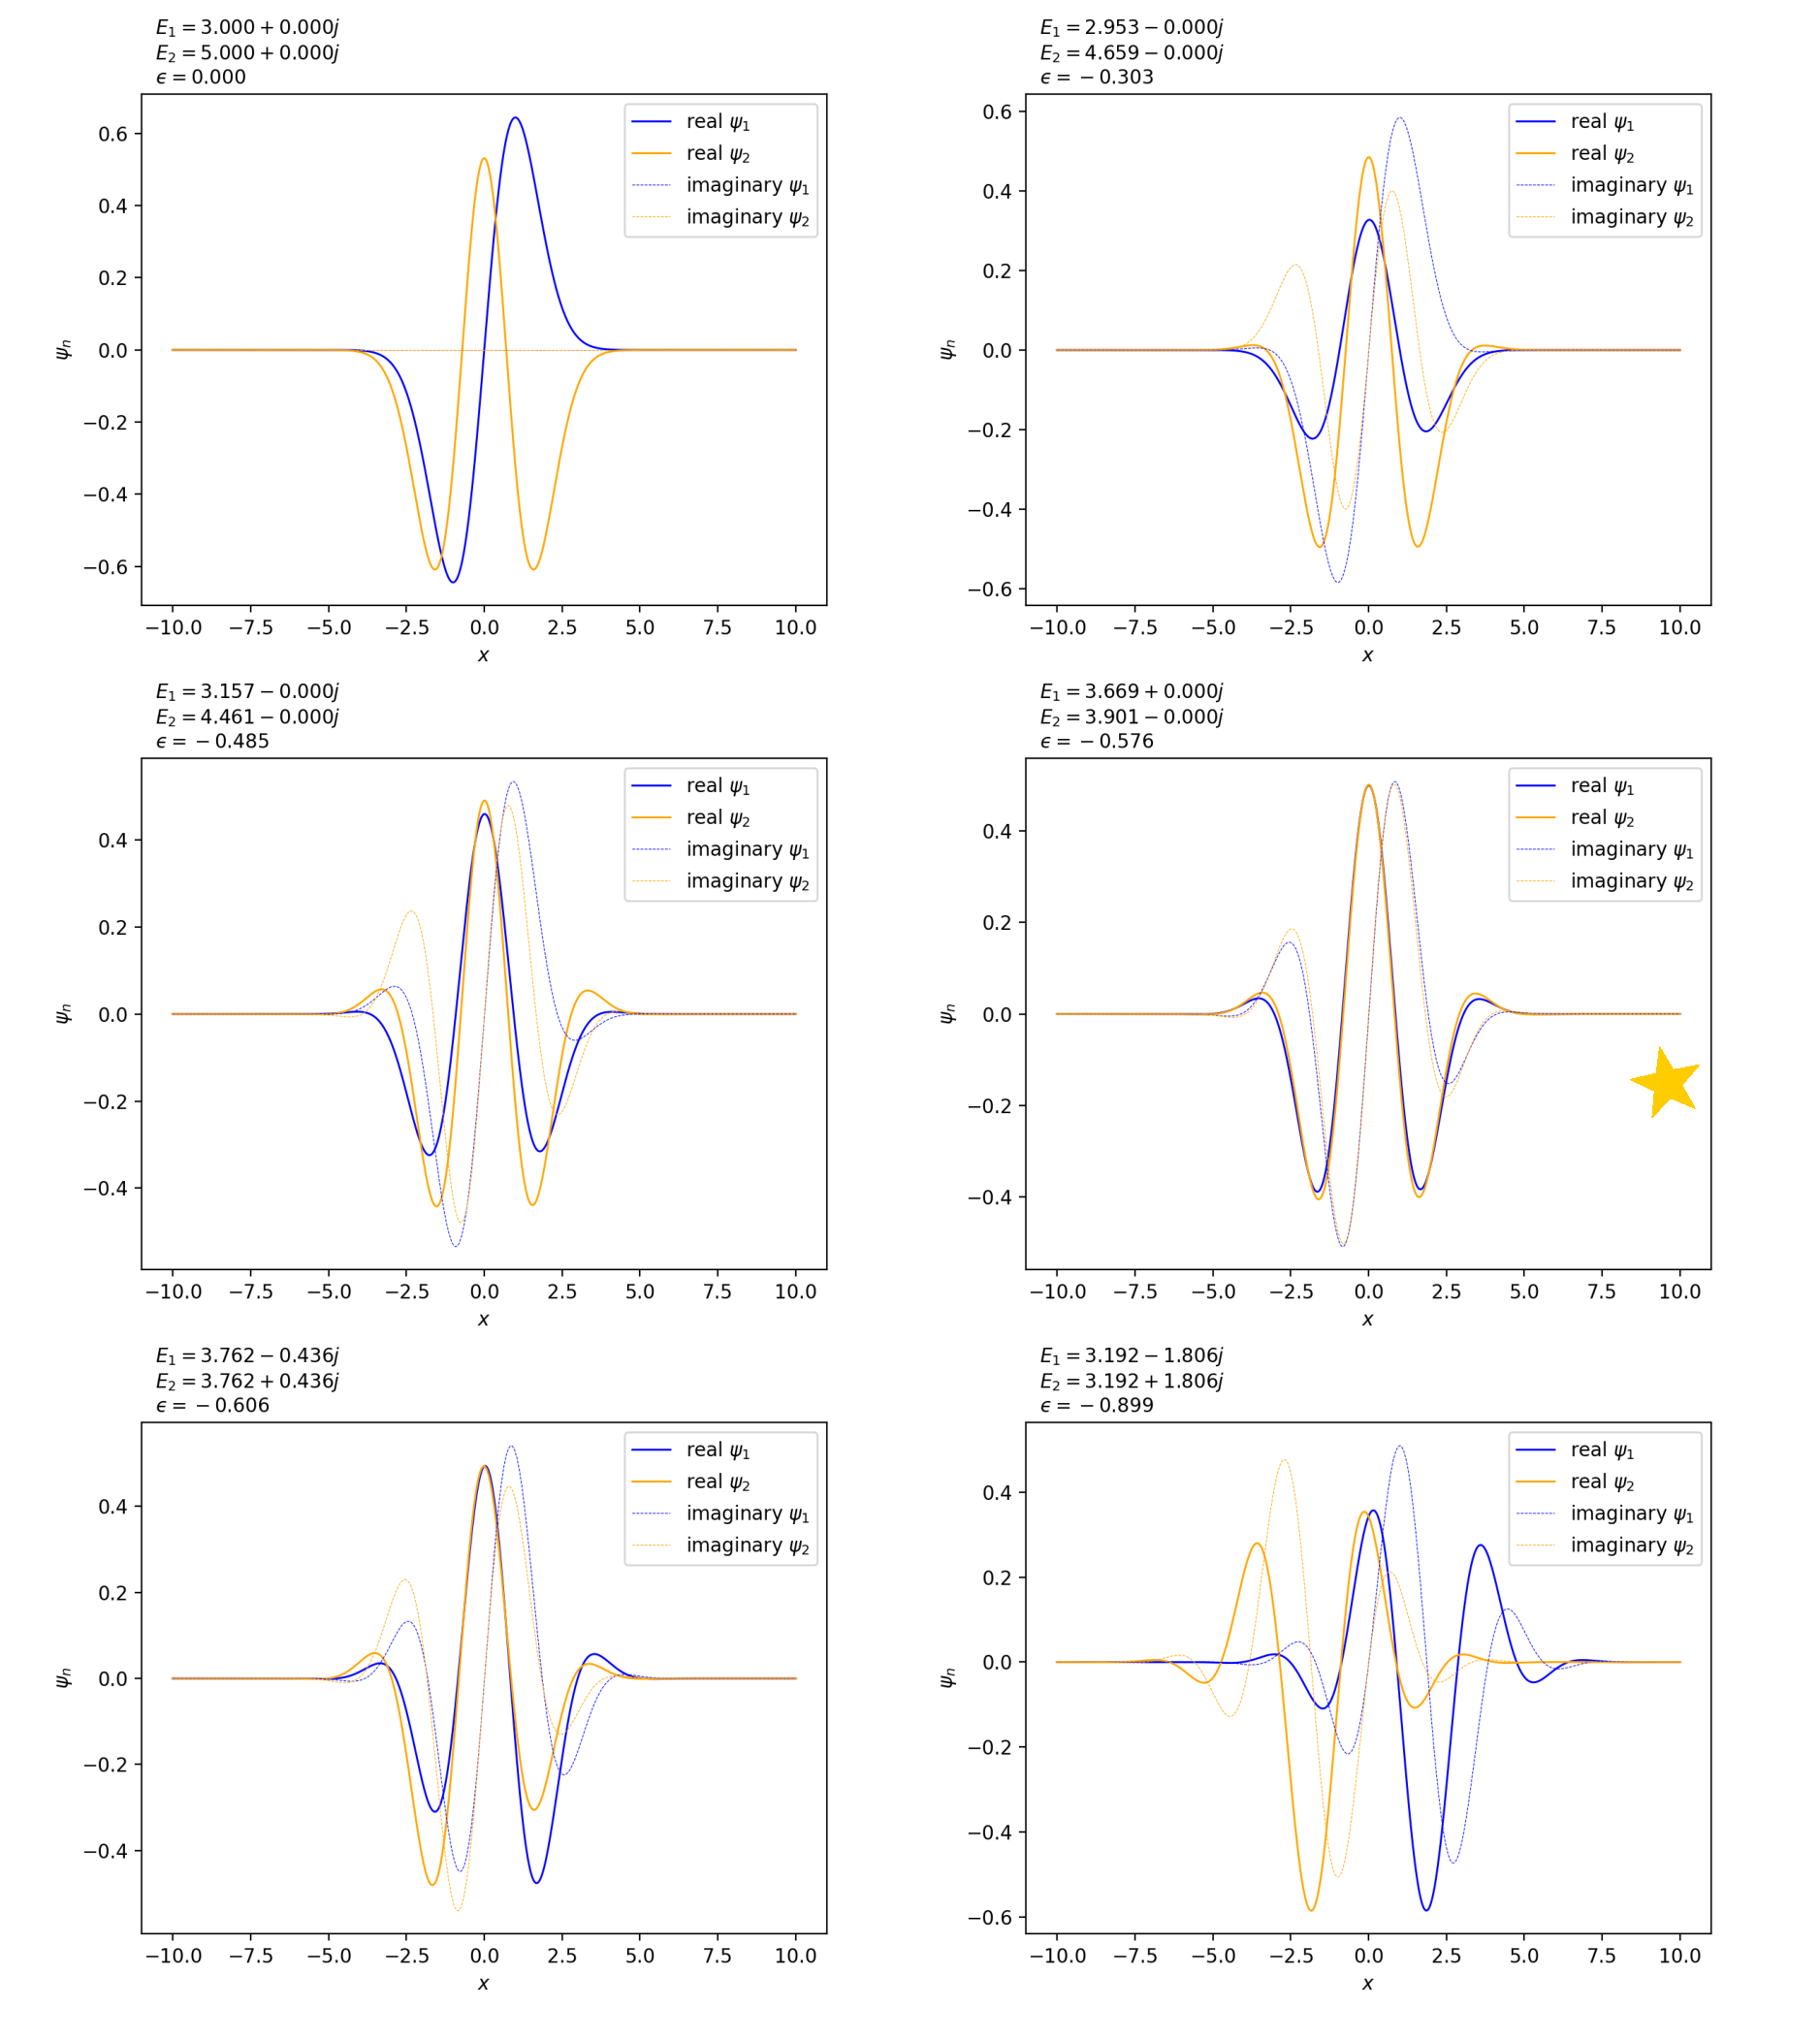
\includegraphics[width=1.1\linewidth]{eigenstates.pdf}
 \captionof{figure}{These are 6 frames in the visualisation of the behaviour of the first and second excited states for the Hamiltonian in equation (\ref{eq:17}) in the region of broken \PT-symmetry. The horizontal axes of each plot represent the $x$ coordinate in a range of -10 to 10, and the vertical axes represent the wave functions $\psi_n(x)$. In addition to the legend I have added on the top left corner of each of the panels the eigenvalues corresponding to each of the first and second excited states ($E_1$ and $E_2$), and the corresponding $\epsilon$ value to make note of this parametric dimension. The panels in this figure should be studied each row from top to bottom from left to right. Here I demonstrate how the structure of the wave function eigenstates changes as we approach the $\epsilon$ value corresponding to the \textbf{exceptional point}. The frame marked with a yellow star corresponds to the value $\epsilon = -0.576$ which is the value closest to the exceptional point that I was able to calculate. in this frame is visible how the wave functions nearly overlap. As $\epsilon$ varies from 0 to -1. At the top left panel, we see that the wave functions plotted are the first and second excited states of the harmonic oscillator, i.e. $\epsilon = 0$.  in the region where $\epsilon$ is less negative than the exceptional point, the wave functions are themselves symmetric about zero. As $\epsilon$ approaches the exceptional point from the left, the wave functions begin to overlap. We can see the wave functions behave as mirror images of each other after $\epsilon$ becomes more negative than the exceptional point.}
\end{Figure}

\begin{Figure}
 \centering
  \hspace*{-0.9cm}
 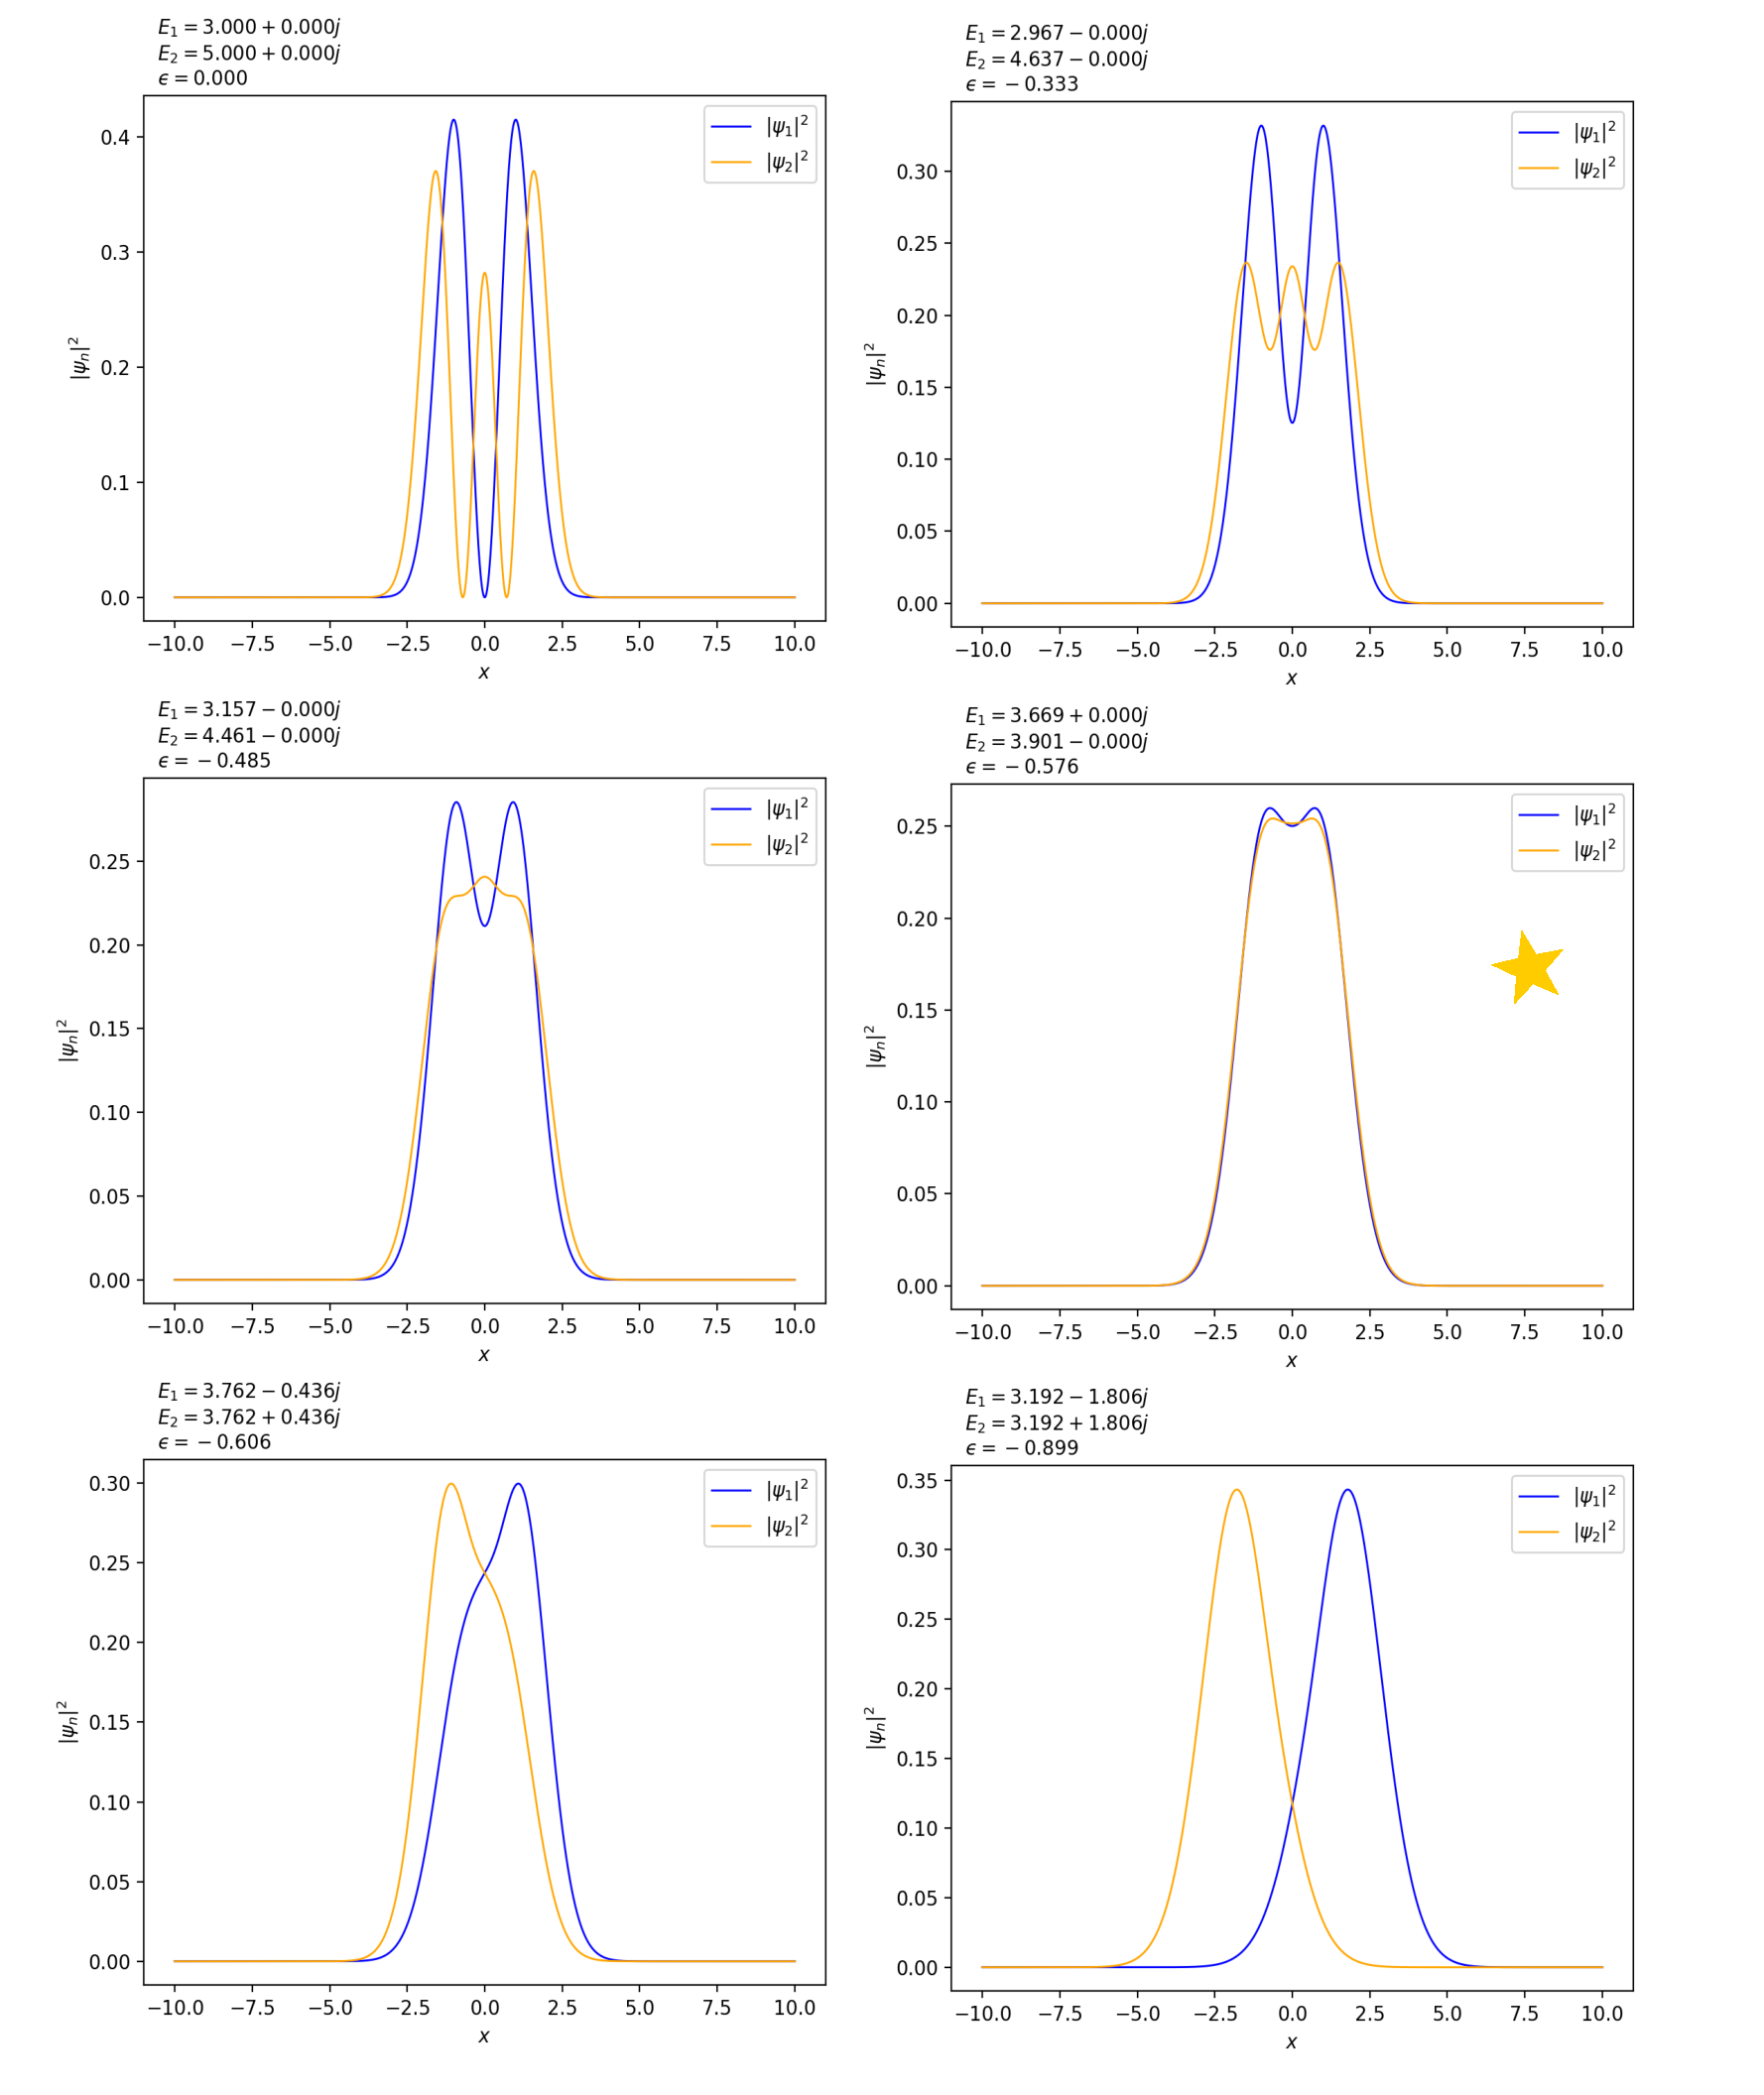
\includegraphics[width=1.1\linewidth]{amplitudes.pdf}
 \captionof{figure}{These are 6 frames in the visualisation of the behaviour of the probability density of the first and second excited states for the Hamiltonian in equation (\ref{eq:17}) in the region of broken \PT-symmetry. Similarly to the previous figure, the horizontal axes of each plot represent the $x$ coordinate in a range of -10 to 10, and the vertical axes represent the probability density of the wave functions $|\psi_n(x)|^{2}$. In addition to the legend I have added on the top left corner of each of the panels the corresponding eigenvalues to each of the first and second excited states ($E_1$ and $E_2$), and the corresponding $\epsilon$ value to make note of this parametric dimension. The panels in this figure should be studied each row from top to bottom from left to right. Here I demonstrate how the structure of the wave function eigenstates changes as we approach the $\epsilon$ value corresponding to the \textbf{exceptional point}. The frame is marked with a yellow star corresponds to the value $\epsilon = -0.576$ which is the value closest to the exceptional point that I was able to calculate. At the top left panel, we see that the probability density of the wave functions are the those corresponding to the first and second excited states of the harmonic oscillator, i.e. $\epsilon = 0$.  in the region where $\epsilon$ is less negative than the exceptional point, the probability densities themselves are symmetric about zero. As $\epsilon$ approaches the exceptional point from the left, the probability densities begin to overlap. We can see the densities of the wave functions behave as mirror images of each other after $\epsilon$ becomes more negative than the exceptional point.}
\end{Figure}

%%%%%%%%%%%%%%%%%%%%%%%%%%%%%%%%%%%%%%%%%%%%%%%%%%%%%%%%%%%%%%%%%%%%%%%%%%%%%%%%%%%%%%%%%%%%%%%%%%%%%%%%%%%%%%%%%%%%%%%%%%%%%%%%%%%%%%%%%%%%%%%%%%%%%%%%%%%%%%%%%%%%%%%%%%%%%

\subsection{The full rendition of Bender's figure}\label{Final}
\begin{Figure}
 \centering
 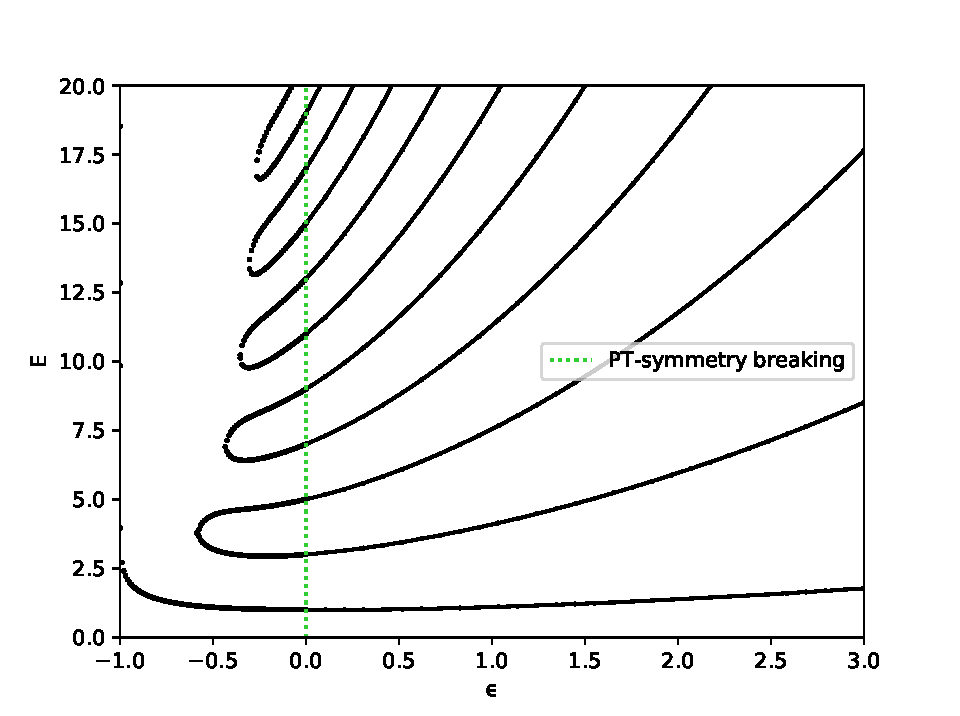
\includegraphics[width=0.75\linewidth]{my_figure_1.pdf}
 \captionof{figure}{My final version of Figure~\ref{fig:Benders} on page~\pageref{fig:Benders}. This figure has all the same characteristics as Bender's original figure.
 All energies presented in this plot are real valued. The $\epsilon$ values are visible in the horizontal axis, while the vertical axis is the energy eigenvalues for each Hamiltonian in the parametric family $\hat{H} = \hat{p}^2 + \hat{x}^2 (i \hat{x})^{\epsilon}$. The vertical dotted green line corresponds to the value $\epsilon = 0$, which itself corresponds to the 1D classical harmonic oscillator Hamiltonian $\hat{H} = \hat{p}^2 + \hat{x}^2$. Above the value $\epsilon = 0$ all values in the spectra are fully real, positive and discrete. Energy levels increase with increasing $\epsilon$. In the region where $0 \geq \epsilon \geq -1$ there is a finite number of real positive eigenvalues and an infinite number of complex-conjugate pairs of eigenvalues (the complex values are not depicted in this figure). The number of real eigenvalues decreases as $\epsilon$ decreases from 0 to -1 , for $\epsilon$ values that are more negative than the value $\epsilon = -0.57793$ the only remaining real eigenvalue corresponds to the ground-state energy. At the value $\epsilon = -1$ the spectrum is null, as all eigenvalues diverge towards positive infinity.}
\end{Figure}

%%%%%%%%%%%%%%%%%%%%%%%%%%%%%%%%%%%%%%%%%%%%%%%%%%%%%%%%%%%%%%%%%%%%%%%%%%%%%%%%%%%%%%%%%%%%%%%%%%%%%%%%%%%%%%%%%%%%%%%%%%%%%%%%%%%%%%%%%%%%%%%%%%%%%%%%%%%%%%%%%%%%%%%%%%%%%

\chapter{Discussion}\label{Discussion}
Since my main project objective became the calculation of the eigenvalues of a family of non-Hermitian, \PT-deformed Hamiltonians, I want to give a bit of an insight on the reasons why I opted for using certain numerical techniques over others.
%%%%%%%%%%%%%%%%%%%%%%%%%%%%%%%%%%%%%%%%%%%%%%%%%%%%%%%%%%%%%%%%%%%%%%%%%%%%%%%%%%%%%%%%%%%%%%%%%%%%%%%%%%%%%%%%%%%%%%%%%%%%%%%%%%%%%%%%%%%%%%%%%%%%%%%%%%%%%%%%%%%%%%%%%%%%%

\section{Complex WKB}\label{Complex WKB}
For the unbroken \PT-symmetry region of the spectrum, I decided to follow Bender's methodology in ``Making sense of non-Hermitian Hamiltonians''. In the paper he describes the WKB approximation technique as yielding a good approximation to the exact energy values of the eigenvalue problem. However, I found its implementation in the complex plane to be quite unintuitive.

The complex WKB method involves treating $x$ as a complex variable (i.e. $x = re^{i\theta}$), and calculating how the asymptotic form of the solutions change as they are traced around the complex plane\cite{Sorrell}. 
Since the integral in the exponent in equation (\ref{eq:21}) is in general, complex valued, the solutions will contain either growing or decaying exponential terms. The nomenclature of the solutions depends on these growing or decaying exponential terms (since they describe a particular asymptotic behaviour). The solutions are called either \textbf{dominant} or \textbf{sub-dominant} depending on these growing or decaying exponential terms respectively.

Note that if the integral in the exponent in equation (\ref{eq:21}) is purely real, then both WKB solutions will be purely oscillatory, with neither dominating the other\cite{Sorrell}.

The bounds ($x_{\pm}$) of the integral in equation (\ref{eq:23}) are turning points of the equation $P(x) = E - V(x)$. Lines can be drawn emanating from the turning points in the complex plane, marking the curves where $\mathrm{Im}(\int_{x_-}^{x^+} P(x)^{\frac{1}{2}}dx) = 0$. These lines are known as \emph{Stokes lines} and they mark the borders between sectors in the complex plane where solutions undergo \textbf{dominant} or \textbf{sub-dominant} behaviour. These sectors are known as \emph{Stokes wedges}. Knowing the position of \emph{Stokes lines} is crucial in applying the complex WKB method\cite{Sorrell}.
%%%%%%%%%%%%%%%%%%%%%%%%%%%%%%%%%%%%%%%%%%%%%%%%%%%%%%%%%%%%%%%%%%%%%%%%%%%%%%%%%%%%%%%%%%%%%%%%%%%%%%%%%%%%%%%%%%%%%%%%%%%%%%%%%%%%%%%%%%%%%%%%%%%%%%%%%%%%%%%%%%%%%%%%%%%%%

\section{\emph{Stokes wedges} and boundary conditions} \label{Boundary conditions}

One aspect of the complex WKB method that I found quite unintuitive was the determination of the boundary conditions for differential equation (\ref{eq:19}).

The WKB method works only for the eigenvalue problems with $\epsilon \geq 0$ because the sub-dominant eigenfunctions vanish exponentially in two \emph{Stokes wedges} in the complex x-plane\cite{BenderPT}.

The \emph{Stokes wedges} I studied are always centred about the origin of the complex x-plane. As I described in section \ref{WKB}, their angular orientation in the complex x-plane can be described by the argument of the complex variable $x = re^{i\theta}$.

The limits of integration used in the WKB technique are analogous to classical turning points. i.e. the total energy of the system obeys the equation $E = x^2 (ix)^{\epsilon}$ and this equation has many complex solutions. However, since we are interested in $E$ being real, we are concerned with what happens to two turning points that lie on the real axis at $\pm \sqrt{E}$ when $\epsilon = 0$ as $\epsilon$ increases\cite{BenderPT}.
The form of the turning points I wrote in equation (\ref{eq:22}) is 
\begin{align} \label{eq:32}
x_{-}& = 
E^{\frac{1}{\epsilon + 2}}
e^{i\theta_{-}}
&\mathrm{and}&
&x_{+} = E^{\frac{1}{\epsilon + 2}} e^{i\theta_{+}},
\end{align}
where the angles are respectively
\begin{align} \label{eq:33}
\theta_{-}& = \frac{4 + 3\epsilon}{4 + 2 \epsilon} \pi
&\mathrm{and}&
&\theta_{+} = - \frac{\epsilon}{4 + 2 \epsilon} \pi.
\end{align}
When $\epsilon$ increases from 0, the turning points move into the complex plane. Notice that these turning points are always symmetric respect to reflections along the imaginary axis. \textbf{This left-right reflection symmetry is the coordinate space realisation of \PT-symmetry}\cite{BenderPT}.

As $\epsilon$ increases from 0, a logarithmic branch-point singularity appears at the origin, and as $\epsilon$ continues increasing in the positive direction, it is necessary to introduce a branch-cut running from the origin along the positive imaginary axis. In this cut plane the solutions to equation (\ref{eq:19}) are analytic and singled-valued\cite{BenderPT}.
\begin{Figure}
 \centering
 \includegraphics[width=0.75\linewidth]{Stokes_wedges.pdf}
 \captionof{figure}{The figure depicts the real-part of x in the horizontal axes, the imaginary-part of x in the vertical axes, a branch cut on the positive-imaginary axes, from zero to imaginary infinity, and four instances of \emph{Stokes wedges} (one red and one yellow to differentiate between them) changing as functions of $\epsilon$. For the cases when $\epsilon > 0$ the opening angles of the sectors decrease and the sectors rotate downward (both changes are respective to the $\epsilon = 0$ case). If $\epsilon = 0$, the angular opening is equal to $\pi/2$ and are centred about the positive-real and the negative-real axis. For the the cases of $\epsilon < 0$ the angular behaviour is opposite to the positive $\epsilon$ values. The wedges get wider and rotate upwards as $\epsilon$ decreases from zero. The changes, get more dramatic for decreasing $\epsilon$ values. In the case of $\epsilon = -1$ the wedges fuse into one along the logarithmic branch cut on the positive-imaginary line. We can describe the topology of this scenario as the logarithmic Riemann surface collapsing onto a single sheet. When this occurs, The spectrum becomes null, meaning that there are no eigenvalues at all\cite{BenderPT}\cite{Bender2017}.}
\end{Figure}
%%%%%%%%%%%%%%%%%%%%%%%%%%%%%%%%%%%%%%%%%%%%%%%%%%%%%%%%%%%%%%%%%%%%%%%%%%%%%%%%%%%%%%%%%%%%%%%%%%%%%%%%%%%%%%%%%%%%%%%%%%%%%%%%%%%%%%%%%%%%%%%%%%%%%%%%%%%%%%%%%%%%%%%%%%%%%

\section{\PT-symmetry breaking}\label{PT breaking}
In the process of fixing several coding errors I made. I was able to explore the WKB integration method more deeply. I investigated the integration contour for the WKB integral by plotting it several times until I identified my integration issues. The Hamiltonian in equation (\ref{eq:17}) can be described as a complex deformed classical harmonic oscillator model, i.e. $H = p^2 + x^2(ix)^{\epsilon}$. Thinking about the Hamiltonian in the non-quantized framework allows us to explore a useful analogy between our integration contour and a particle moving in classical trajectory. When $\epsilon$ assumes non-zero values $H$ deforms into the complex domain\cite{BenderPT}. If $\epsilon \geq 0$ the classical particle trajectories are closed loops, and when $\epsilon < 0$ the trajectories are open paths. This transition at $\epsilon = 0$ is the underlying cause of our observed transition between broken and unbroken \PT-symmetry at the value $\epsilon = 0$.
\begin{Figure}
 \centering
 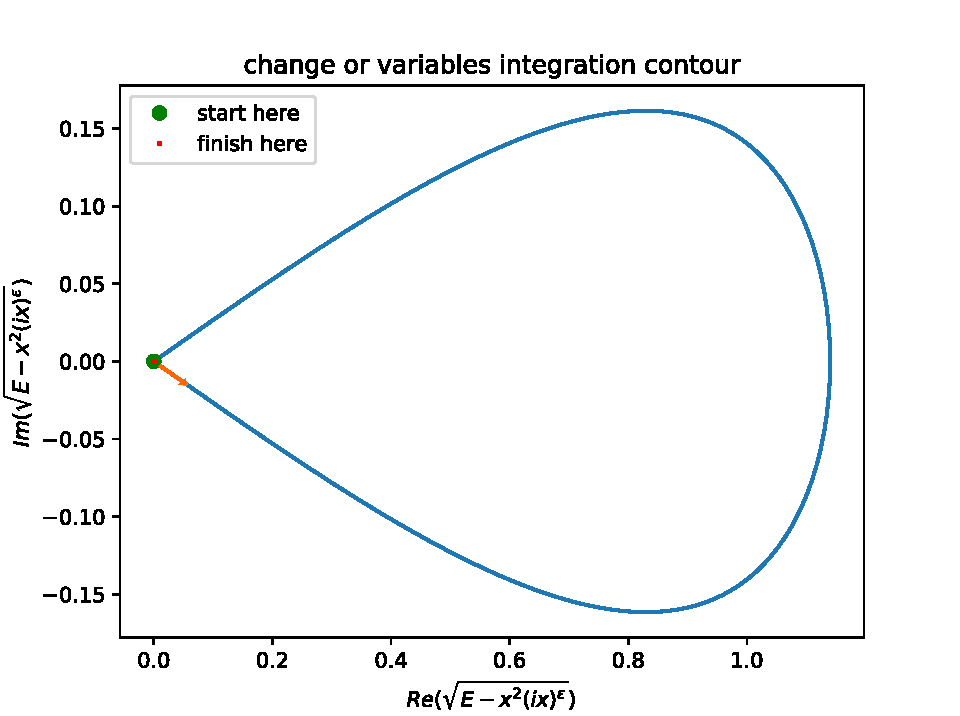
\includegraphics[width=0.75\linewidth]{integration_contour.pdf}
 \captionof{figure}{Integration contour used in my implementation of the WKB method for the region $\epsilon \geq 0$, the real-part of the integrand is the horizontal axis, and the imaginary-part of the integrand is on the vertical axis. The turning point $x_{-}$ is marked in green and the turning point $x_{+}$ is marked in red. I also mark the direction of integration along the contour as an orange arrow along the blue contour. The contour is continuous and closed within the complex x-plane.}
\end{Figure}
I explained in section \ref{WKB} that to use the WKB approximation, it is necessary to impose $\psi \rightarrow 0$ as $|x| \rightarrow \infty$ along the integration contour located within two angular sectors in the complex x-plane. We encounter a problem as $\epsilon$ becomes negative, because in this case there is no continuous path joining the limits of integration used in the WKB approximation, therefore we cannot use this technique in the region with broken \PT-symmetry.

My original idea to solve the eigenvalue problem in the region corresponding to $\epsilon < 0$ was based on the shooting method\cite{N_R}. Unfortunately this idea was difficult to implement given that I was dealing with a complex equation.Since both the wavefunctions and the energies live and so it was not exactly clear to me how I should use this method in the two-dimensional complex plane, it was not exactly clear to me how I should use the shooting method. Eventually, I opted to discretise the range $0 < \epsilon \geq -1$ and proceeded to solve the eigenvalue problems for each resulting parametric Hamiltonian as a matrix equation.

I faced a few complications using the matrix diagonalisation method. Initially my intuition was that the matrices should be dimensionally large so I would get more resolution in the Harmonic oscillator space. This intuition was based on the idea that with more eigenstates come more degrees of freedom and this means that my eigenvalue calculations of the non-Hermitian Hamiltonians would be more accurate. One issue relating to this was that if I increased the number of states used to make my matrix the number of eigenvalues would increase linearly with N and since I only needed to have the first few eigenvalues, this would have been a large computational time waste. The eigenvalue output from my code was a list or disordered eigenvalues. Therefore, the more eigenvalues in my output, the more eigenvalues I had to sort in my list. Given this, I had to devise a way to sort the eigenvalues in order with increasing energy, to later plot only the lowest ones. This issue was one of the reasons why my code was not the fastest, in addition to reasons explained in section \ref{Matrix equations}.
%%%%%%%%%%%%%%%%%%%%%%%%%%%%%%%%%%%%%%%%%%%%%%%%%%%%%%%%%%%%%%%%%%%%%%%%%%%%%%%%%%%%%%%%%%%%%%%%%%%%%%%%%%%%%%%%%%%%%%%%%%%%%%%%%%%%%%%%%%%%%%%%%%%%%%%%%%%%%%%%%%%%%%%%%%%%%

\section{Exceptional points}\label{EPs}

Using complex analysis when studying Hamiltonians demonstrates that energy quantization has a topological interpretation. When we extend the parameters of a Hamiltonian into the complex domain, we find that the energy eigenvalues are all branches of a multivalued function, they are analytic continuations of one another and can be continuously deformed into one another by varying the parameters. Energy levels are in a one to one correspondence with the sheets of a Riemann surface. From the narrow perspective of real variables, this topological interpretation is invisible\cite{BenderPT}. 

The behaviour of the eigenvalues of the Hamiltonian in equation (\ref{eq:18}) for the $\epsilon < 0$ region is a great demonstration of this. Note that there are $\epsilon$ values at which a minimum of two eigenvalues merge (the order of the degeneracy depends on the number of coalescent eigenvalues at that point\cite{BenderPT}\cite{Bender2017}), at $\epsilon = -1$ both Figure~\ref{fig:Benders} on page~\pageref{fig:Benders}, and my own renditions in sections \ref{PT broken} and \ref{Final} display an infinite-order exceptional point.
%%%%%%%%%%%%%%%%%%%%%%%%%%%%%%%%%%%%%%%%%%%%%%%%%%%%%%%%%%%%%%%%%%%%%%%%%%%%%%%%%%%%%%%%%%%%%%%%%%%%%%%%%%%%%%%%%%%%%%%%%%%%%%%%%%%%%%%%%%%%%%%%%%%%%%%%%%%%%%%%%%%%%%%%%%%%%

\subsection{Experimental consequences of non-Hermitian degeneracies}\label{Experimental}
Energy levels follow closed paths in the complex energy plane, however if the closed path encircles an \textbf{exceptional point} (branch-point singularity), the energy levels exchange their identities because they are analytic continuations of one another\cite{BenderPT}\cite{Bender2017}. This phenomenon is called level crossing. Interestingly, it is possible to vary the parameters of a Hamiltonian in laboratory experiments and thus to observe experimentally the effect of encircling exceptional points\cite{Bender2017}. An example of this kind of experimental non-Hermitian degeneracy manipulation can be found in in reference \cite{Ostrovskaya} by Gao et al (2015).
%%%%%%%%%%%%%%%%%%%%%%%%%%%%%%%%%%%%%%%%%%%%%%%%%%%%%%%%%%%%%%%%%%%%%%%%%%%%%%%%%%%%%%%%%%%%%%%%%%%%%%%%%%%%%%%%%%%%%%%%%%%%%%%%%%%%%%%%%%%%%%%%%%%%%%%%%%%%%%%%%%%%%%%%%%%%%

\section{Final remarks}\label{Future}
I have previously explained that when a non-Hermitian Hamiltonian satisfies unbroken \PT-symmetry the energy spectrum of the Hamiltonian in question has all real eigenvalues. \emph{Does this mean that the Hamiltonian I studied can be used to describe actual physics?} The short answer is \textbf{yes}. The long answer requires that we discover an appropriate inner product determined by the \PT-symmetric non-Hermitian Hamiltonian in question. In Bender's words: ``\PT-symmetric quantum mechanics is kind of a \emph{bootstrap} theory in the sense that the Hamiltonian operator $\hat{H}$ chooses the Hilbert space (and associated inner product) in which it prefers to live''\cite{BenderPT}.
%%%%%%%%%%%%%%%%%%%%%%%%%%%%%%%%%%%%%%%%%%%%%%%%%%%%%%%%%%%%%%%%%%%%%%%%%%%%%%%%%%%%%%%%%%%%%%%%%%%%%%%%%%%%%%%%%%%%%%%%%%%%%%%%%%%%%%%%%%%%%%%%%%%%%%%%%%%%%%%%%%%%%%%%%%%%%

\subsection{Orthogonality of eigenfunctions}\label{Orthogonal}
I described my work on the eigenstates wave functions of the Hamiltonian in equation (\ref{eq:17}) in section \ref{Eigenstates}. I mentioned that I wanted to verify if the eigenstates of a particular $\epsilon$ dependent Hamiltonian were orthogonal or not. I wrote some testing code to iteratively plot the density of the wave functions for the Hamiltonians corresponding to $\epsilon = -0.7$, $\epsilon = -0.4$. From these plots I discovered that at least for each of these these values of non-Hermitian Hamiltonians with broken \PT-symmetry there were several non-orthogonal eigenstates, which I verified by plotting wave functions and calculating inner products (see the figure below). This is an interesting finding given that non-orthogonality is highly unusual for eigenstates, at least with respect to the conventional Hermitian inner product.
\begin{Figure}
 \centering
 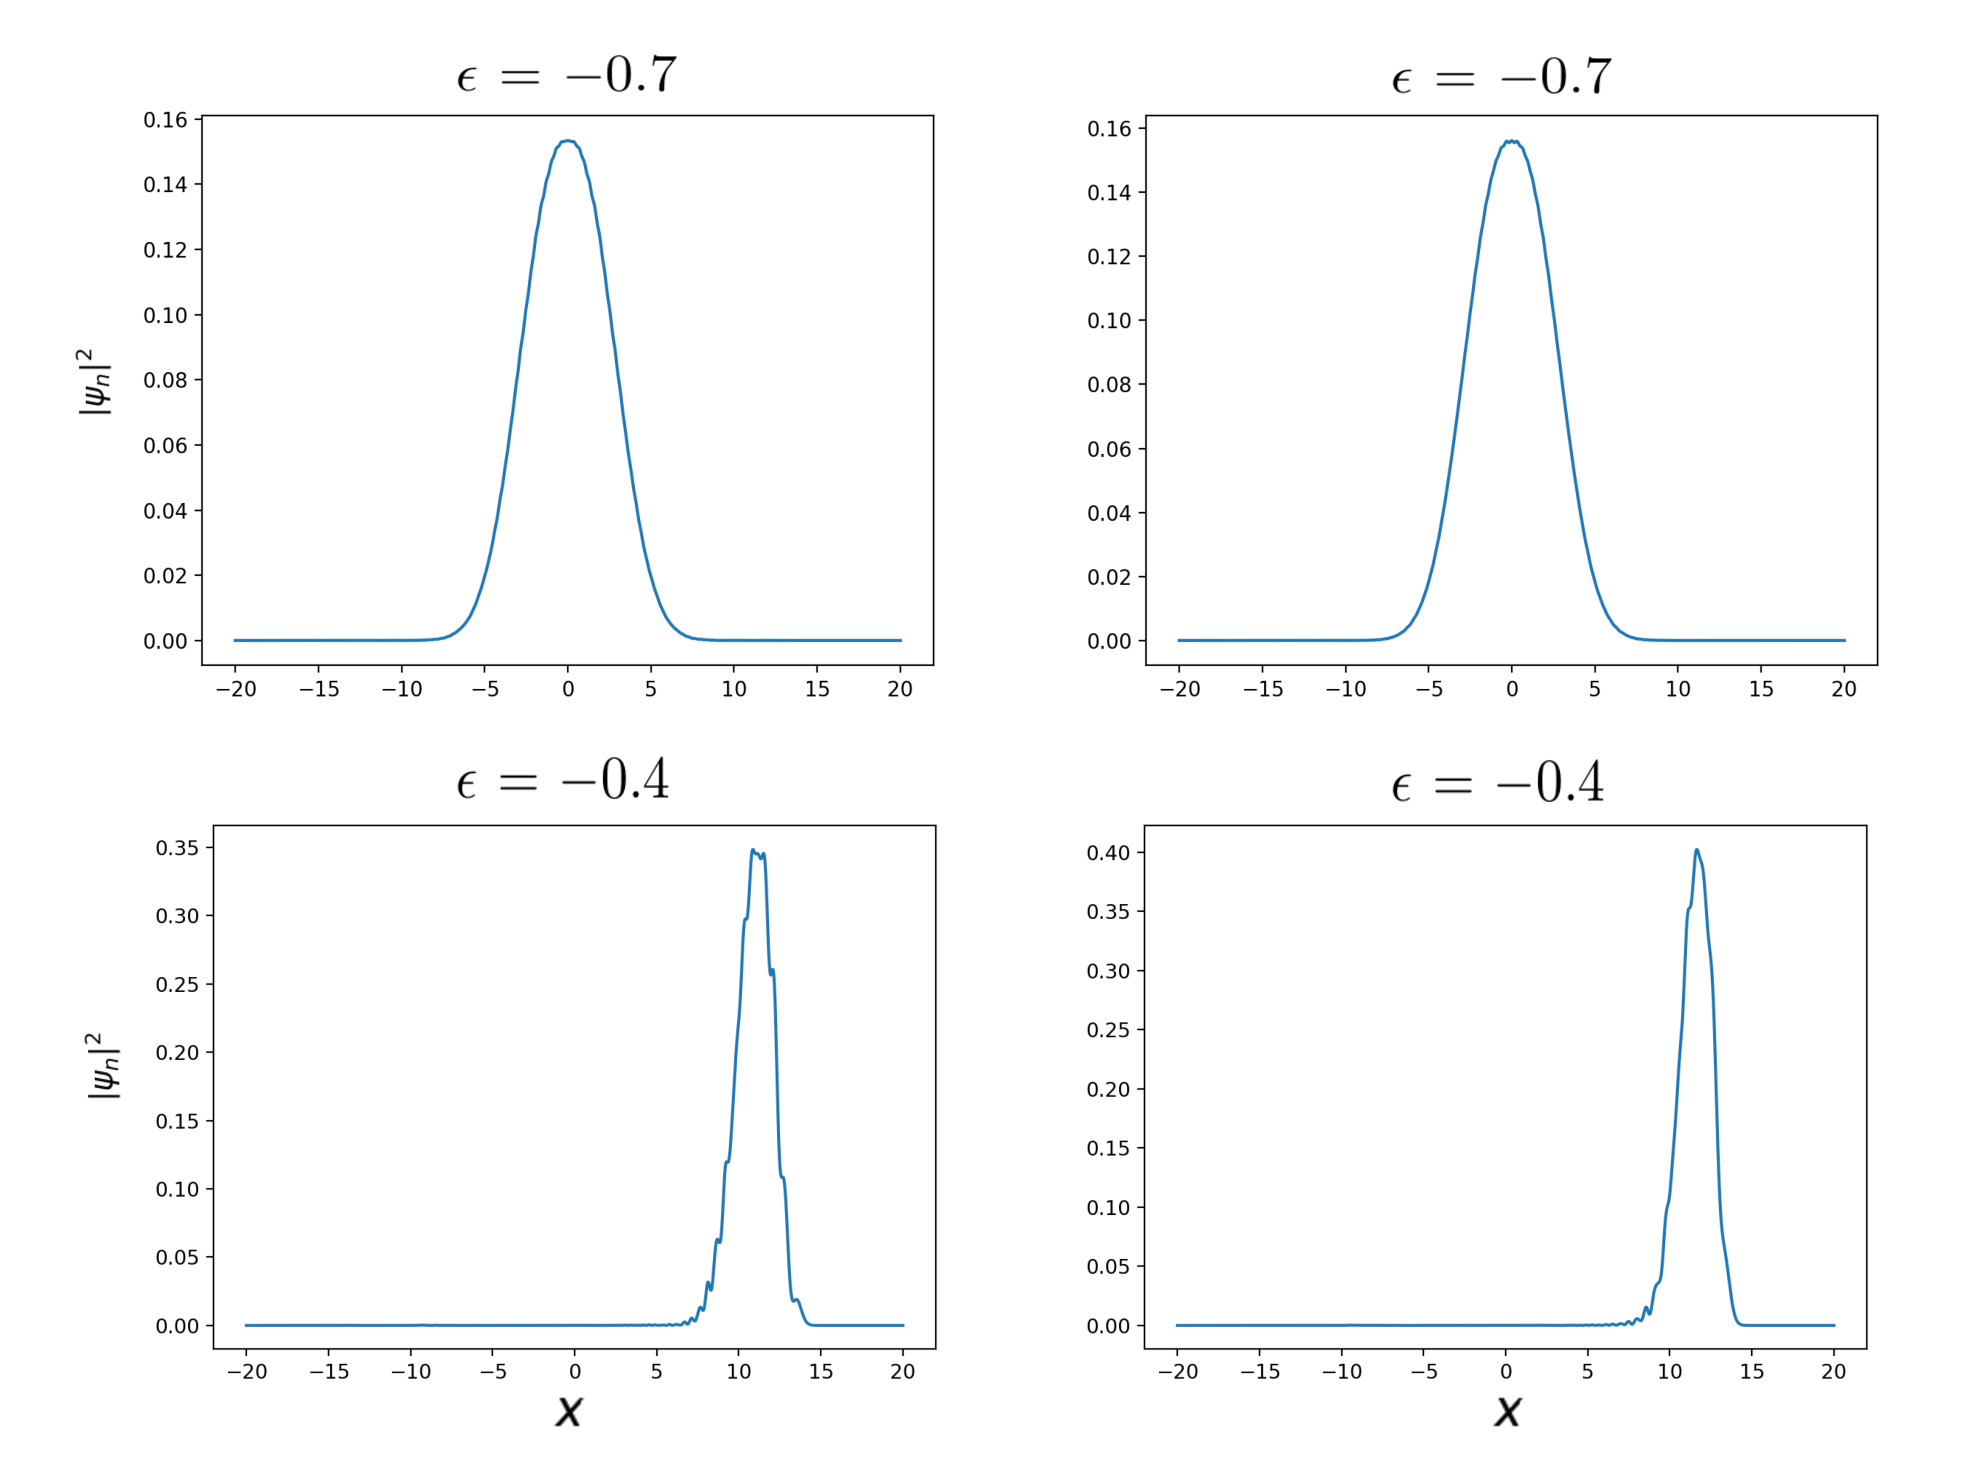
\includegraphics[width=0.8\linewidth]{wavefunctions_-0.4_-0.7.pdf}
 \captionof{figure}{These are 4 plots of the probability density of two eigenstates corresponding to two parametric Hamiltonians belonging to the family in equation (\ref{eq:17}). The horizontal axes of each plot represent the $x$ coordinate in a range of $-20$ to $20$, and the vertical axes represent the probability density of the normalised wave functions. The first row from top to bottom in this matrix of plots displays the probability densities for two wave functions of the Hamiltonian \mbox{$\hat{H} = \hat{p}^2 + \hat{x}^2 (i\hat{x})^{-0.7}$}. The second row in this matrix of plots displays the probability densities for two wave functions of the Hamiltonian \mbox{$\hat{H} = \hat{p}^2 + \hat{x}^2 (i\hat{x})^{-0.4}$}. I chose these wave function density pairs for each of the Hamiltonians because they visually appeared to be non-orthogonal. In addition, I calculated the inner products of each of these wave functions and I confirmed numerically that these functions are not orthogonal. The inner product corresponding to the two wave functions in the top row is $\langle \psi_{39} | \psi_{40} \rangle =-0.7817 + i 3.9907 \times 10^{-10}$. The inner product corresponding to the two wave functions in the bottom row is $\langle \psi_{39} | \psi_{40} \rangle = 0.1846 - i 0.7007$.}
\end{Figure}

A pair of vectors may be orthogonal with respect to one inner product but not respect to another. In the standard formalism of quantum mechanics inner products are assumed to satisfy conjugate transposition and bi-linearity. \\Bi-linearity means that for any vectors $u, v$ in a vector space, $u, v$ must satisfy\cite{Jones-Smith} 
\begin{equation}
\begin{split}
&(i)\ (u, v + w) = (u, v) + (u, w) \mathrm{\ and\ } (u + v, w) = (u, w) + (v, w),\\
&(ii)\ (u, cv) = c(u, v) \mathrm{\ where\ } c \in \mathds{R},\\
&(iii)\ (cu, v) = c^*(u, v).
\end{split}
\end{equation}
It is also required that the inner product of a vector with itself be positive,
and be zero in the case that one of the vectors is the zero vector. Such inner-products are called positive definite\cite{Jones-Smith}.
If we make an educated guess for the form of the inner product based on the role of \PP\ and \TT\ operators in the non-Hermitian formalism of quantum mechanics our guessed inner product might look something like this
\begin{equation}
(u, v) \equiv \int_C dx [u(x)]^{PT} v(x) = \int_C dx [u(-x)]^*v(x),
\end{equation}
where $C$ is a contour that begins and terminates in the \emph{Stokes wedges} used to impose the boundary conditions of our eigenvalue equation. However with this definition we obtain some negative-norm states, deeming our guess inadequate for use in quantum theory\cite{BenderPT}\cite{Jones-Smith}\cite{Moiseyev}.\\
An inner product that results in positive norm states for unbroken \PT-symmetric non-Hermitian Hamiltonians can be found, but it requires that we define a new non-trivial linear operator known as the \emph{C} operator. Unfortunately, this topic was beyond my research at this time.

I conclude this very brief introduction of \PT-symmetric quantum mechanics by reiterating that \PT-symmetric quantum mechanics is a rapidly evolving field that shows great promise as an expansion of what is considered to be ``the most reliable theory ever devised by humankind''.


%%%%%%%%%%%%%%%%%%%%%%%%%%%%%%%%%%%%%%%%%%%%%%%%%%%%%%%%%%%%%%%%%%%%%%%%%%%%%%%%%%%%%%%%%%%%%%%%%%%%%%%%%%%%%%%%%%%%%%%%%%%%%%%%%%%%%%%%%%%%%%%%%%%%%%%%%%%%%%%%%%%%%%%%%%%%%

\chapter{Conclusion}\label{Conclusion}
 In this work I reproduced a figure depicting the eigenvalue spectra of a family of non-Hermitian \PT-symmetric Hamiltonians. The figure demonstrates how the broken or unbroken \PT-symmetry of Hamiltonians affects the boundedness and reality of eigenvalues in their energy spectra. In the figure, several non-Hermitian spectral degeneracies known as exceptional points are shown. I also created a visualisation of the behaviour of two wave function eigenstates for the family of parametric Hamiltonians. In this visualisation it is possible to see how the structure of the wave functions changes in the regions of broken \PT-symmetry. By varying the parameter that characterizes the Hamiltonians and approaching a parametric value corresponding to an exceptional point, I demonstrate the that the structure of wave functions are themselves symmetric about zero before crossing the exceptional point and the wave functions behave as mirror images of each other in the parametric region past the exceptional point value. The aim of this project report is to add evidence for the thesis on the robustness of Non-Hermitian quantum mechanics as an extension to quantum theory. Non-Hermitian quantum theory is based on the redefinition of the Hermicity condition expected for operators in quantum mechanics. If only Hermicity is replaced by \PT-symmetry but all other postulates of quantum theory are preserved, the number of possible systems available to study using quantum theory is expanded.
%%%%%%%%%%%%%%%%%%%%%%%%%%%%%%%%%%%%%%%%%%%%%%%%%%%%%%%%%%%%%%%%%%%%%%%%%%%%%%%%%%%%%%%%%%%%%%%%%%%%%%%%%%%%%%%%%%%%%%%%%%%%%%%%%%%%%%%%%%%%%%%%%%%%%%%%%%%%%%%%%%%%%%%%%%%%%

\chapter{Acknowledgements}\label{Acknowledgements}
I want to thank my supervisors Jesper and Meera for giving me their time and for guiding me through the semester with great ideas and suggestions. I truly enjoyed all of the moments when we met to discuss physics and other topics. I also want to thank our research group members for being so welcoming, asking tough questions and for giving me helpful suggestions for my oral presentation. I am also grateful to Daniel Price for giving me the opportunity to try out research in a formal setting by accepting my request to join this research unit and for being so attentive and responsive to my emails. Lastly, I want to thank my partner Chris for being an endless source of inspiration, helpful advice and for all our interesting rants and discussions. 

\begin{center}
\vspace{5cm}
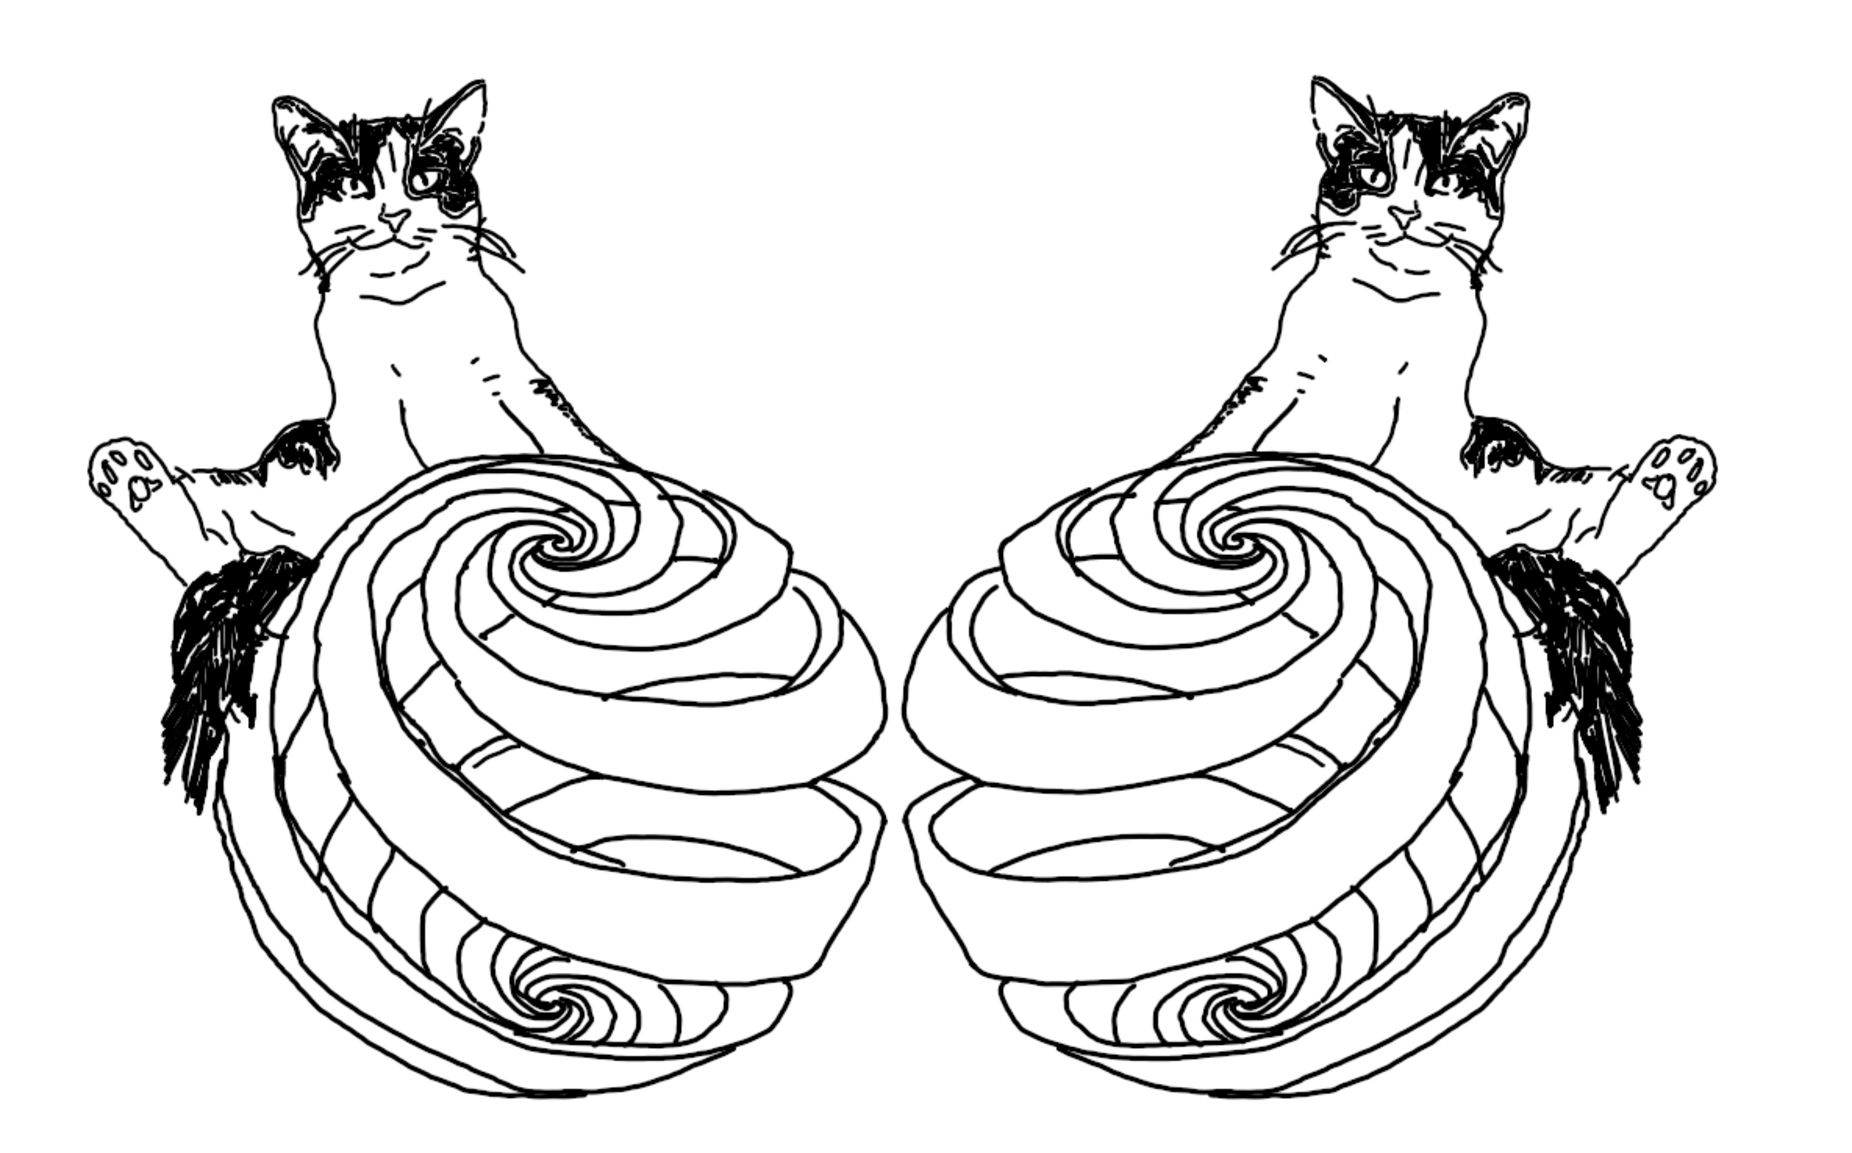
\includegraphics[scale=0.2]{bepqed.pdf}
% \vspace{10cm}
\end{center}
%%%%%%%%%%%%%%%%%%%%%%%%%%%%%%%%%%%%%%%%%%%%%%%%%%%%%%%%%%%%%%%%%%%%%%%%%%%%%%%%%%%%%%%%%%%%%%%%%%%%%%%%%%%%%%%%%%%%%%%%%%%%%%%%%%%%%%%%%%%%%%%%%%%%%%%%%%%%%%%%%%%%%%%%%%%%%

\chapter{Appendix}\label{Appendix}
\section{Time dependent wave packet simulation}\label{Aborted}
\subsection{Methods}
This section closely follows ``Non-Hermitian quantum mechanics'' by Nimrod Moiseyev. A book that I was referred to by my supervisors early on in the semester. The numerical propagation of wave packets is simpler when taken within the framework of non-Hermitian quantum mechanics rather than in the standard (Hermitian) formalism\cite{Moiseyev}. The main idea behind this method is to include a reflection-free complex absorbing potential (RF-CAP) in the Hamiltonian describing the wave packet's time evolution. This added potential term allows the description of outward flowing states without any un-physical reflection effects from the boundary of the simulation region.

I was very eager to verify this technique on a simulation of a wave packet propagating in space using Python. First, I constructed a wave function to be propagated in space and time. Since I required analytically verifiable derivatives, I figured that the easiest wave function choice was a Gaussian wave packet with initial condition 
\begin{equation} \label{eq:13}
\psi(x, 0) = e^{-(x^2/2\sigma^2)}e^{ik_{0}x},
\end{equation}
where I set $x \in \mathds{R}$, $\sigma = 1$ and $k_{0} = 10$. In order to implement the time evolution of my wave function, I used the 1D Schrödinger equation
 \begin{equation} \label{eq:14}
\frac{d}{dt}\psi(x, t) = \frac{-i}{\hbar} \left [ \frac{-\hbar^2}{2m} \frac{d^2}{dx^2} + V(x, t)\right ] \psi(x, t),
\end{equation}
To numerically calculate the second order spatial derivative, I used the Fourier transform property \\\mbox{$\mathcal{F}\{f'(x)\} = ik\mathcal{F}\{f(x)\}$}, therefore my equation became
\begin{equation} \label{eq:15}
f(x, t, \psi) = \frac{-i}{\hbar} \left [ \frac{-\hbar^2}{2m} \mathcal{F}^{-1}\{-k^2\mathcal{F}\{\psi(x, t)\}\} + V(x, t)\psi(x, t)\right ],
\end{equation}
I was originally unsure of what the potential $V(x,t)$ should look like since the whole point of this exercise is the inclusion of a reflection-free complex absorbing potential (RF-CAP) in the potential of the Hamiltonian. The RF-CAP should attain non-zero values only in the boundary region in the coordinate space where the physical potential $V(x,t)$ vanishes\cite{Moiseyev}. Eventually, I opted for implementing a square well potential as $V(x,t)$ to give rise to the required non-physical interference that should be expected at the spatial boundaries of this problem.
I defined the square well potential V(x, t) as an array over an x-array ranging from $0$ to $10$. The square potential was defined as zero everywhere in the x-array except at the boundaries. The boundaries' height was determined by trial and error based on the kinetic energy of the wave packet. I settled with having the barrier to be a thousand times larger than the initial value for the wave vector squared, \mbox{i.e. $V(0, t) = V(10, t) = 1000k_0^2$}.

To implement the time evolution required by the simulation I used fourth-order Runge-Kutta on equation (\ref{eq:15}). The Runge-Kutta algorithm is defined as\cite{N_R}
\begin{equation} \label{eq:16}
\begin{split}
&k_1 = f(x, t, \psi),\\
&k_2 = f(x, t + \frac{\Delta t}{2}, \psi + \frac{1}{2}k_1),\\
&k_3 = f(x, t + \frac{\Delta t}{2}, \psi + \frac{1}{2}k_2),\\
&k_4 = f(x, t + \Delta t, \psi + k_3),\\
&\psi_{n + 1} = \psi_{n} + \frac{1}{6}(k_1 + 2k_2 + 2k_3 + k_4) + O(\Delta t^5).\\
\end{split}
\end{equation}
where I set $\Delta t = 0.0001$ as the evolution time step, I chose this value to be small enough to be able to resolve motion of the Nyquist mode within the spatial step 
$\Delta x = \frac{x_{\mathrm{max}} - x_{\mathrm{min}}}{1024} = \frac{10}{1024}$.
The numerical formula in equation (\ref{eq:16}) propagates a solution over a time interval, by solving a differential equation using four Euler-style steps, i.e. the $k_i$ coefficients (each Euler-style step involves one evaluation of the differential equation with slightly different parameters), and then combining the information obtained for each solution to match a Taylor series expansion up to fourth order. By combining the evaluations of the differential equation in this way we eliminate the error terms order by order, leaving the error remaining being very small\cite{N_R}.
%%%%%%%%%%%%%%%%%%%%%%%%%%%%%%%%%%%%%%%%%%%%%%%%%%%%%%%%%%%%%%%%%%%%%%%%%%%%%%%%%%%%%%%%%%%%%%%%%%%%%%%%%%%%%%%%%%%%%%%%%%%%%%%%%%%%%%%%%%%%%%%%%%%%%%%%%%%%%%%%%%%%%%%%%%%%%

\subsection{Results}
\begin{Figure}
\centering
\vspace*{-0.9cm}
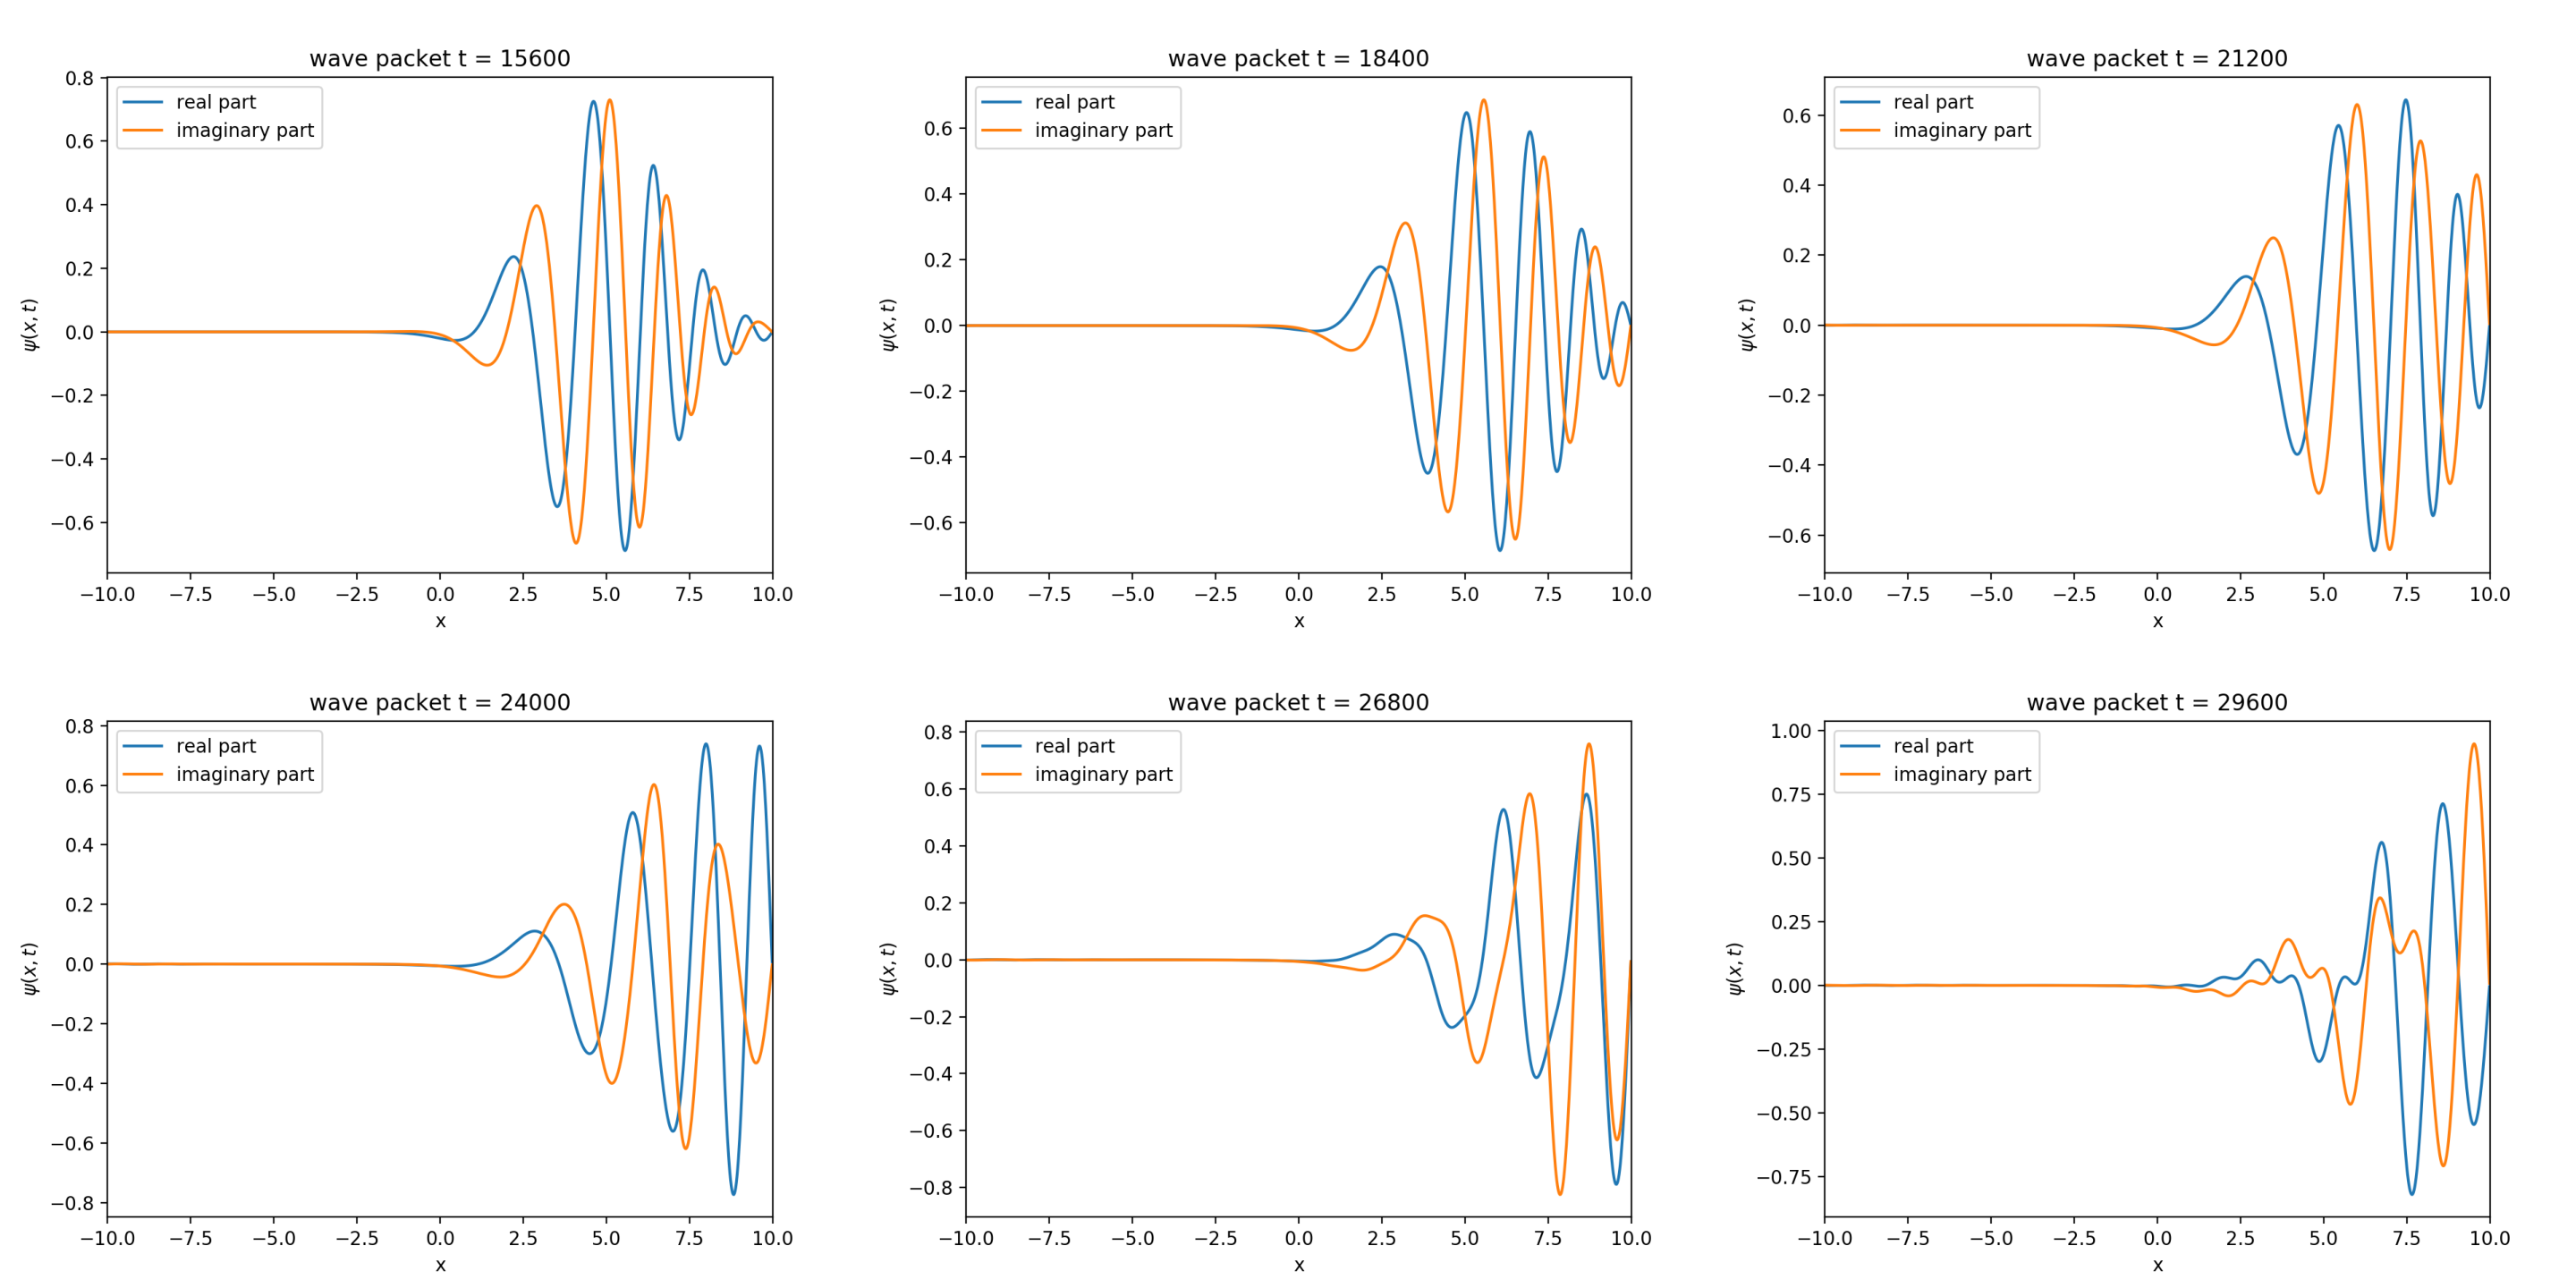
\includegraphics[width=\linewidth]{propagating_wave_with_reflection.pdf}
\captionof{figure}{These are 6 frames of my simulation of a right propagating Gaussian wave packet in space as a function of time. The horizontal axes of every frame correspond to the spatial coordinate x (dimensionless) and the vertical axes of every frame correspond to the real and imaginary parts of the Gaussian wave packet. The earliest time frame is the top left panel, corresponding to the wave packet position at time t = 15600 as can be seen in that panel's title. The panels in this figure should be studied from left to right and top to bottom. An ``undesirable'' reflection of the wave packet interacting with the boundary is visible specially in the latest 3 frames corresponding to times t = 24000, t = 26800 and t = 29600 as can be seen in those panels' titles.}
\end{Figure}
Understanding the implementation of the potential characteristic to this non-Hermitian simulation technique required a lot of reading and I ambitiously decided to leave this sub-project unfinished in the meantime and continue with it after I successfully replicated Figure 1. in Bender, a sub-project which I naively expected to finish quickly.
%%%%%%%%%%%%%%%%%%%%%%%%%%%%%%%%%%%%%%%%%%%%%%%%%%%%%%%%%%%%%%%%%%%%%%%%%%%%%%%%%%%%%%%%%%%%%%%%%%%%%%%%%%%%%%%%%%%%%%%%%%%%%%%%%%%%%%%%%%%%%%%%%%%%%%%%%%%%%%%%%%%%%%%%%%%%%

% %----------------------------------------------------------------------------------------
% %   ABBREVIATIONS
% %----------------------------------------------------------------------------------------

% % \begin{abbreviations}{ll} % Include a list of abbreviations (a table of two columns)

% % \textbf{LAH} & \textbf{L}ist \textbf{A}bbreviations \textbf{H}ere\\
% % \textbf{WSF} & \textbf{W}hat (it) \textbf{S}tands \textbf{F}or\\

% % \end{abbreviations}

\bibliography{mybib}
\bibliographystyle{unsrt}
\end{document}